%%% LaTeX-Vorlage Version 1.4 %%%
\documentclass[a4paper,fontsize=11pt,oneside,parskip=half,headings=normal]{scrreprt} 
% \usepackage{showframe} % nur für Kontrolle der Ränder 

%%% Präambel einbinden %%%
%%% Präambel %%%
% hier sollten keine Änderungen erforderlich sein
%
\usepackage[utf8]{inputenc}   % Zeichencodierung UTF-8 für Eingabe-Dateien
\usepackage[T1]{fontenc}      % Darstellung von Umlauten im PDF

\usepackage{svg}
\usepackage{tabularx}
\usepackage[bottom]{footmisc}
\usepackage{listings}         % für Einbindung von Code-Listings
\lstset{numbers=left,numberstyle=\tiny,numbersep=5pt,texcl=true}
\lstset{literate=             % erlaubt Sonderzeichen in Code-Listings 
{Ö}{{\"O}}1
{Ä}{{\"A}}1
{Ü}{{\"U}}1
{ß}{{\ss}}2
{ü}{{\"u}}1
{ä}{{\"a}}1
{ö}{{\"o}}1
{€}{{\euro}}1
}

\usepackage[
  inner=35mm,outer=15mm,top=25mm,
  bottom=20mm,foot=12mm,includefoot
]{geometry}                 % Einstellungen für Ränder

\usepackage[english]{babel} % Spracheinstellungen Englisch
\usepackage[babel,english=british]{csquotes} % deutsche Anf.zeichen
\usepackage{enumerate}      % anpassbare Nummerier./Aufz.
\usepackage{graphicx}       % Einbinden von Grafiken
\usepackage[onehalfspacing]{setspace} % anderthalbzeilig

\usepackage{blindtext}      % Textgenerierung für Testzwecke
\usepackage{color}          % Verwendung von Farbe 

\usepackage{acronym}        % für ein Abkürzungsverzeichnis

\usepackage[                % Biblatex
  backend=biber,
  bibstyle=_dhbw_authoryear,
  citestyle=authoryear,
  uniquename=true, useprefix=true,
  bibencoding=utf8]{biblatex}
%kein Punkt am Ende bei \footcite
%http://www.golatex.de/footcite-ohne-punkt-am-schluss-t4865.html
\renewcommand{\bibfootnotewrapper}[1]{\bibsentence#1}


%Reihenfolge der Autorennamen
%   
% http://golatex.de/viewtopic,p,80448.html#80448
% Argumente: siehe http://texwelt.de/blog/modifizieren-eines-biblatex-stils/
\DeclareNameFormat{sortname}{% Bibliographie
  \ifnum\value{uniquename}=0 % Normalfall
    \ifuseprefix%
      {%
         \usebibmacro{name:family-given}
           {\namepartfamily}
           {\namepartgiveni}
           {\namepartprefix}
           {\namepartsuffixi}%
       }
      {%
         \usebibmacro{name:family-given}
           {\namepartfamily}
           {\namepartgiveni}
           {\namepartprefixi}
           {\namepartsuffixi}%
       }%
  \fi
  \ifnum\value{uniquename}=1% falls nicht eindeutig, abgek. Vorname 
      {%
         \usebibmacro{name:family-given}
           {\namepartfamily}
           {\namepartgiveni}
           {\namepartprefix}
           {\namepartsuffix}%
       }%
  \fi
  \ifnum\value{uniquename}=2% falls nicht eindeutig, ganzer Vorname 
      {%
         \usebibmacro{name:family-given}
           {\namepartfamily}
           {\namepartgiven}
           {\namepartprefix}
           {\namepartsuffix}%
       }%
  \fi   
  \usebibmacro{name:andothers}}

\DeclareNameFormat{labelname}{% für Zitate
  \ifnum\value{uniquename}=0 % Normalfall
    \ifuseprefix%
      {%
         \usebibmacro{name:family-given}
           {\namepartfamily}
           {\empty}
           {\namepartprefix}
           {\namepartsuffixi}%
       }
      {%
         \usebibmacro{name:family-given}
           {\namepartfamily}
           {\empty}
           {\namepartprefixi}
           {\namepartsuffixi}%
       }%
  \fi
  \ifnum\value{uniquename}=1% falls nicht eindeutig, abgek. Vorname 
      {%
         \usebibmacro{name:family-given}
           {\namepartfamily}
           {\namepartgiveni}
           {\namepartprefix}
           {\namepartsuffix}%
       }%
  \fi
  \ifnum\value{uniquename}=2% falls nicht eindeutig, ganzer Vorname 
      {%
         \usebibmacro{name:family-given}
           {\namepartfamily}
           {\namepartgiven}
           {\namepartprefix}
           {\namepartsuffix}%
       }%
  \fi   
  \usebibmacro{name:andothers}}
      
  
\DeclareFieldFormat{extrayear}{% = the 'a' in 'Jones 1995a'
  \iffieldnums{labelyear}
    {\mknumalph{#1}}
    {\mknumalph{#1}}}        

\renewcommand*{\multinamedelim}{\addslash}
\renewcommand*{\finalnamedelim}{\addslash}
\renewcommand*{\multilistdelim}{\addslash}
\renewcommand*{\finallistdelim}{\addslash}

\renewcommand{\nameyeardelim}{~}

% Literaturverzeichnis: Doppelpunkt zwischen Name (Jahr): Rest 
% http://de.comp.text.tex.narkive.com/Tn1HUIXB/biblatex-authoryear-und-doppelpunkt
\renewcommand{\labelnamepunct}{\addcolon\addspace}

% Im Literaturverzeichnis: Autor (Jahr) fett
\renewbibmacro*{author}{%
  \ifboolexpr{%
    test \ifuseauthor%
    and
    not test {\ifnameundef{author}}
  }
    {\usebibmacro{bbx:dashcheck}
       {\bibnamedash}
       {\usebibmacro{bbx:savehash}%
        \textbf{\printnames{author}}%
        \iffieldundef{authortype}
          {\setunit{\addspace}}
          {\setunit{\addcomma\space}}}%
     \iffieldundef{authortype}
       {}
       {\usebibmacro{authorstrg}%
        \setunit{\addspace}}}%
    {\global\undef\bbx@lasthash
     \usebibmacro{labeltitle}%
     \setunit*{\addspace}}%
  \textbf{\usebibmacro{date+extrayear}}}

% Sonderfall: Quelle ohne Autor, aber mit Herausgeber
% Name des Herausgebers wird fett gedruckt
\renewbibmacro*{bbx:editor}[1]{%
  \ifboolexpr{%
    test \ifuseeditor%
    and
    not test {\ifnameundef{editor}}
  }
    {\usebibmacro{bbx:dashcheck}
       {\bibnamedash}
       {\textbf{\printnames{editor}}%
        \setunit{\addcomma\space}%
        \usebibmacro{bbx:savehash}}%
     \usebibmacro{#1}%
     \clearname{editor}%
     \setunit{\addspace}}%
    {\global\undef\bbx@lasthash
     \usebibmacro{labeltitle}%
     \setunit*{\addspace}}%
  \textbf{\usebibmacro{date+extrayear}}}

% Anpassungen für deutsche Sprache
\DefineBibliographyStrings{ngerman}{%
	nodate = {{o.J.}},
	urlseen = {{Abruf:}},
	ibidem = {{ebenda}}
}

% Benennung der Verzeichnisse
\defbibheading{lit}{\section*{List of literature}}
\defbibheading{www}{\section*{List of Internet and intranet sources}}
\defbibheading{gespraeche}{\section*{List of conversations}}

% Anpassungen für die englische Sprache
\DefineBibliographyStrings{english}{
    nodate = {{w.y.}},
    urlseen = {{retrieval:}}
} % mit DHBW-spezifischen Einstellungen

\usepackage{hyperref}       % URL-Formatierung, klickbare Verweise

\usepackage{tocloft}        % für Verzeichnis der Anhänge

\newcounter{anhcnt}
\setcounter{anhcnt}{0}
\newlistof{anhang}{app}{}

\newcommand{\anhang}[1]{%
  \refstepcounter{anhcnt}
  \setcounter{anhteilcnt}{0}
  \section*{Appendix \theanhcnt: #1}
  \addcontentsline{app}{section}{\protect\numberline{A.\theanhcnt}#1}\par
}

\newcounter{anhteilcnt}
\setcounter{anhteilcnt}{0}

\newcommand{\anhangteil}[1]{%
	\refstepcounter{anhteilcnt}
	\subsection*{Appendix~\arabic{anhcnt}/\arabic{anhteilcnt}: #1}
	\addcontentsline{app}{subsection}{\protect\numberline{A.\theanhcnt/\arabic{anhteilcnt}}#1}\par
}

\renewcommand{\theanhteilcnt}{Appendix \theanhcnt/\arabic{anhteilcnt}}

\usepackage{chngcntr}                % fortlaufende Zähler für Fußnoten, Abbildungen und Tabellen
\counterwithout{figure}{chapter}
\counterwithout{table}{chapter}
\counterwithout{footnote}{chapter}

\usepackage[automark]{scrlayer-scrpage} 
%% Definitionen für Kopf- und Fußzeile auf normalen Seiten
\defpagestyle{kopfzeile}
{% Kopfdefinition
  (\textwidth,0pt)    % Länge der oberen Linie,Dicke der oberen Linie       
  {} % Definition für linke Seiten im doppelseitigen Layout
  {} % Definition für rechte Seiten im doppelseitigen Layout      
  {  % Definition für Seiten im einseitigen Layout
	\makebox[0pt][l]{\rightmark}% 
	\makebox[\linewidth]{}% 
  }        
  (\textwidth, 0.4pt) % Untere Linienlänge, Untere Liniendicke
}
{% Fußdefinition
  (\textwidth,0pt)    % Obere Linienlänge, Obere Liniendicke
  {} % Definition für linke Seiten im doppelseitigen Layout
  {} % Definition für rechte Seiten im doppelseitigen Layout
  {  % Definition für Seiten im einseitigen Layout
    \makebox[\linewidth]{}%
    \makebox[0pt][r]{\pagemark}%
  }
  (\textwidth, 0pt)   % Länge der unteren Linie,Dicke der unteren Linie
}

%% Definitionen für Kopf- und Fußzeile auf ersten Seiten eines Kapitels
\defpagestyle{kapitelkopfzeile}
{% Kopfdefinition
  (\textwidth,0pt)    % Länge der oberen Linie,Dicke der oberen Linie       
  {} % Definition für linke Seiten im doppelseitigen Layout
  {} % Definition für rechte Seiten im doppelseitigen Layout      
  {}  % Definition für Seiten im einseitigen Layout
  (\textwidth, 0pt) % Untere Linienlänge, Untere Liniendicke
}
{% Fußdefinition
  (\textwidth,0pt)    % Obere Linienlänge, Obere Liniendicke
  {} % Definition für linke Seiten im doppelseitigen Layout
  {} % Definition für rechte Seiten im doppelseitigen Layout
  {  % Definition für Seiten im einseitigen Layout
    \makebox[\linewidth]{}%
    \makebox[0pt][r]{\pagemark}%
  }
  (\textwidth, 0pt)   % Länge der unteren Linie,Dicke der unteren Linie
}

%% Definitionen für Kopf- und Fußzeile im Anhang und bei Quellenverzeichnisse
\newcommand{\spezialkopfzeileBezeichnung}{}
\defpagestyle{spezialkopfzeile}
{% Kopfdefinition
  (\textwidth,0pt)    % Länge der oberen Linie,Dicke der oberen Linie       
  {} % Definition für linke Seiten im doppelseitigen Layout
  {} % Definition für rechte Seiten im doppelseitigen Layout      
  {  % Definition für Seiten im einseitigen Layout
	\makebox[0pt][l]{\spezialkopfzeileBezeichnung}% 
	\makebox[\linewidth]{}% 
  }        
  (\textwidth, 0.4pt) % Untere Linienlänge, Untere Liniendicke
}
{% Fußdefinition
  (\textwidth,0pt)    % Obere Linienlänge, Obere Liniendicke
  {} % Definition für linke Seiten im doppelseitigen Layout
  {} % Definition für rechte Seiten im doppelseitigen Layout
  {  % Definition für Seiten im einseitigen Layout
    \makebox[\linewidth]{}%
    \makebox[0pt][r]{\pagemark}%
  }
  (\textwidth, 0pt)   % Länge der unteren Linie,Dicke der unteren Linie
}
            
\newcommand\spezialkopfzeile[1]{%
  \renewcommand\spezialkopfzeileBezeichnung{#1}
  \pagestyle{spezialkopfzeile}
}                 
                  
% Standard-Pagestyle auswählen
\pagestyle{kopfzeile}

% keine Kopfzeile anzeigen auf Seiten, auf denen ein 
% Kapitel beginnt oder das Inhalts-/Abbildungs-/Tabellenverzeichnis steht 
\renewcommand{\chapterpagestyle}{kapitelkopfzeile}
\tocloftpagestyle{kapitelkopfzeile}

		 % für schöne Kopfzeilen 

\usepackage{textcomp}			 % erlaubt EUR-Zeichen in Eingabedatei
\usepackage{eurosym}             % offizielles EUR-Symbol in Ausgabe
\renewcommand{\texteuro}{\euro}  % ACHTUNG: nach hyperref aufrufen!

\usepackage{scrhack}             % stellt Kompatibilität zw. KOMA-Script
                                 % (scrreprt) und anderen Paketen her
                                 
% Anpassung der Abstände bei Kapitelüberschriften
% (betrifft auch Inhalts-, Abbildungs- und Tabellenverzeichnis)
\renewcommand*\chapterheadstartvskip{\vspace*{-\topskip}}
\newcommand{\myBeforeTitleSkip}{1mm}
\newcommand{\myAfterTitleSkip}{10mm}
\setlength\cftbeforetoctitleskip{\myBeforeTitleSkip}
\setlength\cftbeforeloftitleskip{\myBeforeTitleSkip}
\setlength\cftbeforelottitleskip{\myBeforeTitleSkip}

\setlength\cftaftertoctitleskip{\myAfterTitleSkip}
\setlength\cftafterloftitleskip{\myAfterTitleSkip}
\setlength\cftafterlottitleskip{\myAfterTitleSkip}                                                            
%%% Ende der Präambel %%%

%%% Name Ihrer Literatur-Datenbank (ggf. anpassen) %%%
\bibliography{includes/literatur-datenbank.bib}

\begin{document}
%%% Deckblatt einbinden %%% 
% Anpassungen nötig (Name, Titel etc.)
% HIER EDITIEREN: 
% Typ der Arbeit (für Deckblatt und ehrenwörtliche Erklärung)
% - bitte Zutreffendes auswählen
%\newcommand{\typMeinerArbeit}{1. Projektarbeit} 
%\newcommand{\typMeinerArbeit}{2. Projektarbeit} 
%\newcommand{\typMeinerArbeit}{Seminararbeit} 
\newcommand{\typMeinerArbeit}{Bachelor thesis} 

% Thema der Arbeit (für ehrenwörtliche Erklärung)
% HIER EDITIEREN: 
\newcommand{\themaMeinerArbeit}{A design science approach to visualize blockchain transactions (for teaching purposes)}

\thispagestyle{empty}

\begin{spacing}{1}
\begin{center}	
~\vspace{0mm}

% HIER EDITIEREN: Titel der Arbeit
{\sffamily
\LARGE  
% \Large  % bei sehr langen Titeln ggf. etwas kleinere Schriftart wählen
\textbf{A design science approach to visualize blockchain transactions (for teaching purposes)}

%\bigskip
%\textbf{ggf. etwas länger}
}


\vspace{15mm}

% HIER EDITIEREN
{\Large \typMeinerArbeit}

\vspace{1cm}

% HIER ggf. EDITIEREN
submitted on May 07, 2018
\vspace{15mm}
Faculty of economics
\medskip

Business informatics degree programme
\medskip

% HIER EDITIEREN: Kurs eintragen
Course WWI2015F

\vspace{10mm}

by

\vspace{10mm}

% HIER EDITIEREN: Vorname und Name eintragen 
{\large\textsc{Lisa Martiny}}

\vspace{10mm}
\end{center}

\vfill

% HIER EDITIEREN
\begin{tabular}{ll}
Responsible person in the training center: & DHBW Stuttgart: \\
\hspace{0.4\linewidth} & \\
HPE & Professor, John Sören Pettersson \\
Ralph Beckmann  &  \\
Blockchain Advisor TS Consulting \\
\\
Sinature \\
\end{tabular}


\vspace{1cm}
%(etwas Platz für die Unterschrift des Betreuers aus der Ausbildungsstätte)
\end{spacing}

% falls ein Sperrvermerk erforderlich ist: 
%\begin{center}
%\small
%\textbf{Sperrvermerk}:
%Der Inhalt dieser Arbeit darf weder als Ganzes noch in Auszügen \\
%Personen außerhalb des Prüfungsprozesses und des Evaluationsverfahrens zugänglich gemacht werden, sofern keine anders lautende Genehmigung der Ausbildungsstätte vorliegt. 
%\end{center}


% HIER EDITIEREN: Meta-Daten für PDF-Datei
\hypersetup{pdftitle={Titel der Arbeit}}
\hypersetup{pdfauthor={Ihr Name}}
\hypersetup{pdfsubject={Bachelorarbeit DHBW Stuttgart 2015}}

%%% Umstellung der Seiten-Nummerierung auf i, ii, iii ... %%%
\pagenumbering{Roman} 

%%% Abstract (optionale Kurzfassung Ihrer Arbeit) %%%
%\begin{abstract}
\thispagestyle{kapitelkopfzeile}
\textbf{\LaTeX-Vorlage für Projekt-, Seminar- und Bachelorarbeiten}

Bei dem vorliegenden Dokument handelt es sich um eine Vorlage, die
für Projekt-, Seminar- und Bachelorarbeiten im Studiengang
Wirtschaftsinformatik der DHBW Stuttgart verwendet werden kann.

Sie setzt die technischen Vorgaben der Zitierrichtlinie des Studiengangs
(Stand: 01/2018) um.

\emph{Hinweis:} Dieses Dokument ersetzt keine Anleitung oder Einführung in \LaTeX,
für die Nutzung sind daher gewisse Vorkenntnisse unerlässlich. Ein Einstieg in 
\LaTeX\ ist aber weniger schwierig, als es vielleicht auf den ersten Blick scheint
und lohnt sich für das Verfassen wissenschaftlicher Arbeiten in jedem Fall.\footnote{%
so auch \url{http://www.spiegel.de/netzwelt/tech/textsatz-keine-angst-vor-latex-a-549509.html}} 

Ihre Rückmeldungen und Anregungen zu dieser Vorlage nehme ich gerne per E-Mail an die Adresse
\url{tobias.straub@dhbw-stuttgart.de} entgegen.

--- Prof. Dr. Tobias Straub

\vspace{5em}

\begin{center}\small
\begin{tabular}{ccl}
\multicolumn{3}{c}{\textbf{Versionshistorie}}\\
\hline
1.0	& 05.02.2015 & erste Fassung \\
\hline
1.1 & 16.02.2015 & siehe~\ref{anhang:ReleaseNotes11} \\
\hline
1.2 & 20.04.2015 & siehe~\ref{anhang:ReleaseNotes12} \\
\hline
1.3 & 20.02.2016 & siehe~\ref{anhang:ReleaseNotes13} \\
\hline
1.4 & 24.07.2017 & siehe~\ref{anhang:ReleaseNotes14} \\
\hline
1.5 & 07.01.2018 & siehe~\ref{anhang:ReleaseNotes15} \\
\end{tabular}
\end{center}

\end{abstract}


%\cleardoublepage

\renewcommand{\listfigurename}{List of figures}
\renewcommand{\listtablename}{List of tables}

%%% Inhalts-, Abbildungs-, Tabellenverzeichnisse %%%
% sollen einzeilig gesetzt werden, um Platz zu sparen 
\begin{spacing}{1}
\tableofcontents
\clearpage
\chapter*{List of abbreviations}
\addcontentsline{toc}{chapter}{List of abbreviations}

Ein Abkürzungsverzeichnis ist optional. Das Paket \verb|acronym| kann weit mehr, als hier gezeigt.\footnote{siehe \url{http://ctan.org/pkg/acronym}}
Beachten Sie allerdings, dass Sie die Einträge selbst in sortierter Reihenfolge angeben müssen.

\begin{acronym}[DHBW] 
% Argument definiert die Breite der ersten Spalte anhand des längsten vorkommenden Eintrags
\acro{CRM}{Customer Relationship Management}
\acro{DHBW}{Duale Hochschule Baden-Württemberg}
\acro{IEEE}{Institute of Electrical and Electronics Engineers}
\acro{ITIL}{IT Infrastructure Library}
\acro{RoI}{Return-On-Invest}
\acro{UCS}{Universal Character Set}
\acro{UTF-8}{8-Bit UCS Transformation Format} 
\end{acronym}

\vspace{2em}
{\footnotesize
\textbf{Ergänzende Bemerkung:}
Eine im Text verwendete Abkürzung sollte bei ihrer ersten Verwendung erklärt werden. Falls Sie sich nicht selbst darum kümmern möchten, kann das das Paket \verb|acronym| übernehmen und auch automatisch Links zum Abkürzungsverzeichnis hinzufügen. Dazu ist an allen Stellen, an denen die Abkürzung vorkommt, \verb|\ac{ITIL}| zu schreiben. 

Das Ergebnis sieht wie folgt aus: 
\begin{itemize}
\item erstmalige Verwendung von \verb|\ac{ITIL}| ergibt: \ac{ITIL},
\item weitere Verwendung von \verb|\ac{ITIL}| ergibt: \ac{ITIL}
\end{itemize}
Wo benötigt, kann man mit dem Befehl \verb|\acl{ITIL}| wieder die Langfassung ausgeben lassen: \acl{ITIL}.

Falls man die Abkürzungen durchgängig so handhabt, kann man durch Paket-Optionen (in \verb|_dhbw_praeambel.tex|)
erreichen, dass im Abkürzungsverzeichnis nur die tatsächlich verwendeten Quellen aufgeführt werden (Option: \verb|printonlyused|) und zu jedem Eintrag die Seite der ersten Verwendung angegeben wird (Option: \verb|withpage|).
}
\clearpage
\thispagestyle{kapitelkopfzeile}
\listoffigures
\addcontentsline{toc}{chapter}{List of figures} % Abb.verz. ins Inh.verz. aufnehmen
\clearpage
\addcontentsline{toc}{chapter}{List of tables}   % Tab.verz. ins Inh.verz. aufnehmen
\listoftables
\end{spacing}

%%% Umstellung der Seiten-Nummerierung auf 1, 2, 3 ... %%%
\cleardoublepage
\pagenumbering{arabic}

%%% Ihr eigentlicher Inhalt %%%
% Empfehlung: strukturieren Sie Ihren Text in einzelnen Dateien 
% und binden Sie diese hier mit \input{includes/dateiname.tex} ein

\chapter{Introduction}
\label{chapter:Intro}

Blockchain technology has seen an enormous rise in interest in the recent years, coming to its climax at the end of 2017. This development is suggested to be mainly driven by the cryptocurrency bitcoin which is the most widely known cryptocurrency in the market and whose value increased from \$900 to \$20.000 within the last year.\footcite[Cf.][]{Higgins900200002017}
However, with the rise in interest, the number of persons wondering \enquote{But what exactly is bitcoin?} and \enquote{What is this blockchain technology?} has also risen. Simple Google search requests for \enquote{\textit{what is bitcoin}} and \enquote{\textit{what is blockchain}} have peaked in December 2017, as illustrated in figure \ref{fig:SearchRequests}, and yield 10.6 million and 3.8 million results. Of these results, the top ones claim to explain the technology in as little words as possible (\enquote{\textit{WTF is The Blockchain?
The ultimate 3500-word guide in plain English to understand Blockchain.}}\footcite{MamoriaWTFBlockchain2017}, \enquote{\textit{Explain Bitcoin Like I'm 5}}\footcite{CustodioExplainBitcoinFive2013}, \enquote{\textit{Blockchain: everything you want to know about the technology but were too embarrassed to ask}}\footcite{HeathmannBlockchaineverythingyou2018}, or \enquote{\textit{Still don't understand the blockchain? This explainer will help}}\footcite{LeighSinodStilldonunderstand2018}), trying to catch the attention of everyone who has not yet understood this technology. In fact, there are various articles, videos, and further resources available online which all try to explain the technology in an easy to understand manner. However, these claims appear to be empty promises, as most of them do not introduce the learner to the overall value of the technology, but instead explain the technical details which constitute the innovation behind this technology. As one expert states, these resources, mostly published by blockchain enthusiasts, \enquote{are too technical [..] and missing the \textit{easy} language},\footcite[Cf.][P19, P20]{DanielKaltenbach_Interview} thus discouraging people with little or no knowledge from learning more about the technology.

\begin{figure}
    \centering
    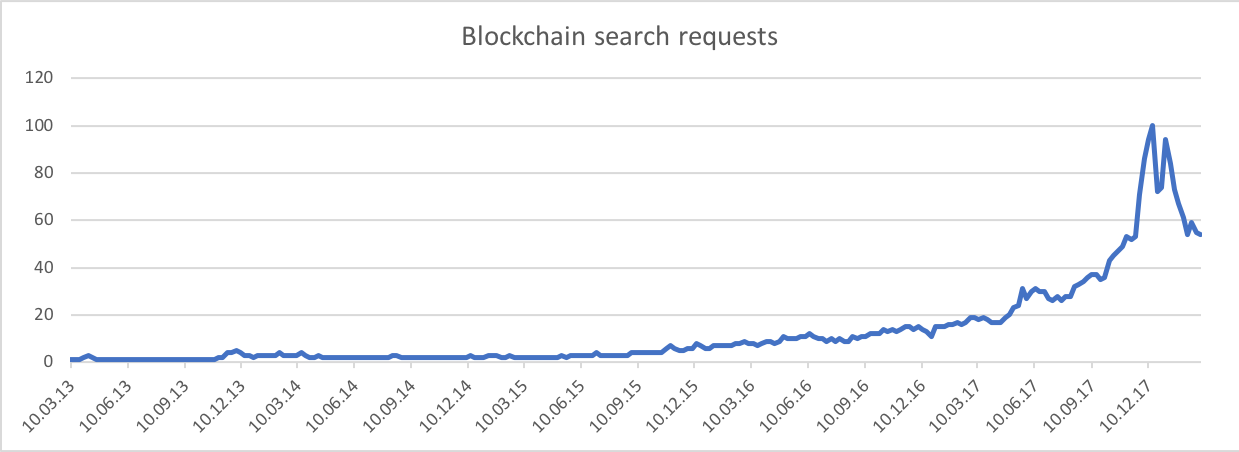
\includegraphics[width=\textwidth]{latex-vorlage_v1.5/graphics/BCRQ.png}
    \caption[Google Trends results for \enquote{blockchain} search requests.]{Google Trends results for \enquote{blockchain} search requests.\protect\footnotemark}
    \label{fig:SearchRequests}
\end{figure}
\footnotetext{Data extracted on the 12th of March, 2018 from https://trends.google.com/trends/explore?date=today\%205-y\&q=\%2Fm\%2F0138n0j1}

However, blockchain offers various opportunities which may improve processes in various industries and enables new, previously impossible business models. Possibly affected industries range from financial services, technology, media, and telecommunications, to energy and resources, life sciences, or health care, as well as the horizontal applications of audit and cybersecurity.\footcite[Cf.][]{SchatskybitcoinBlockchaincoming2015} Unfortunately, only few companies show interest in applying this technology to their business at the time of writing. This may be because many do not yet fully understand the technology and are missing an appropriate explanation which provides real and pithy examples.\footcite[Cf.][P88]{BjoernPaulewicz_Interview}

% https://moguldom.com/14060/100-of-the-best-quotes-on-bitcoin-and-blockchain/
% “Every informed person needs to know about Bitcoin because it might be one of the world’s most important developments.”

% –Leon Luow, Nobel Peace prize nominee 

\section{Problem statement} \label{sec:Problem}
\chapquote{Writing a description for this thing for general audiences is bloody hard. There's nothing to relate it to.}{Satoshi Nakamoto}{Creator of Bitcoin\footcite{NakamotoReSlashdotSubmission2010}}

This quote by Satoshi Nakamoto, the creator of bitcoin, describes the problem this paper wants to resolve. 
With regard to the numerous attempts of explaining the blockchain technology, it may be argued that there are so many different, yet very similar explanations because writing a good explanation is difficult and the different authors feel that other articles do not adequately master this task. In addition, the blockchain technology is sophisticated, as it builds on a variety of different topics, such as cryptography, game theory, computer networking, data transmission as well as monetary theory, complicating this task even more.\footcite[Cf.][]{LoppNobodyUnderstandsBitcoin2017} 

Due to the high interest in this technology by the general public and the various application fields in different industries, this paper argues it is essential to provide the public with an easy to understand introduction. Such an introduction should allow the audience to transfer the given information to their field of work and imagine how the technology may be of use in their situation. %The paper is further motivated by the hypothesis that if a professional understands the blockchain technology and the value it may deliver, they are more open to implementing it in their business and might take advantages of the organization's consulting services regarding the blockchain technology.
Additionally, a well rounded and simple introduction to this topic would be useful for the organization's employees as well, as they would be able to gain an overview of the possible use cases without needing to read or access numerous other learning resources.

\section{Objective and scope} \label{sec:Objective}

The objective of this paper is, therefore, to create an artifact which introduces a novice audience to the blockchain technology. This introduction should be readily accessible to the general audience, it should not require any prior knowledge, and it should convey the information in a more engaging way than the existing learning resources. The research question, which leads this research from here forward is, therefore, the question: \textbf{What and how should the artifact visualize information, so it explains the blockchain technology in a comprehensible way to a novice audience?}

Following the design science research method, this paper develops an artifact (an instantiation) aiming to solve this problem. To define the solution space, expert interviews are conducted and analyzed according to Mayring's qualitative content analysis. As research in information systems includes the study of people,\footcite[Cf.][p.11]{OsterleGestaltungsorientierteWirtschaftsinformatikPladoyer2010} Mayer's cognitive theory of multimedia instructions gives additional insights into how an explanation should be structured. In how far Mayer's theory is correct is out of scope for this paper. This paper does also not cover every minute detail of the blockchain technology. Instead, it focuses on the most important concepts which are crucial components of the blockchain and its various use cases, as the final artifact presents only the most relevant information. 
    
\section{Thesis overview} \label{sec:ThesisOverview}
The thesis communicates the results of the design science research process in the following structure: Following the introduction in chapter \ref{chapter:Intro}, the blockchain technology is presented. Chapter \ref{chap:Blockchain} gives an overview of the overall technology, situates it in the context of cryptoeconomics (the three underlying concepts of finance, economics, and information technology (\acs{IT})) and presents possible use cases. The following chapter \ref{chapter:Multimedia} then presents Mayer's cognitive theory of multimedia learning, describes which role interactivity plays in the learning process, and finally lists the guidelines to be followed when designing multimedia instructions. It is then followed by a thorough discussion of design science research (chapter \ref{chap:DesignScience}, which begins with placing the research method in the context of information systems research, before describing the components and the process of design science. Chapter \ref{chap:ReqEng} then presents how the requirements for the solution space are gathered. Various experts within the organization are interviewed, and their responses are presented. Additionally to these interviews, the chapter reviews existing solutions (with a focus on interactive blockchain visualizations) which also serve as input to the requirements elicitation process. On the basis of this input, chapter \ref{chapter:Solution} then defines the solution space, by which the artifact is designed and developed in chapter \ref{chap:designanddev}. After that, chapter \ref{chap:Evaluation} presents the implementation of the artifact for an exemplary demonstration and its evaluation. The results are discussed and possible improvements are listed. The paper then concludes with chapter \ref{chap:conclusion} which reflects on the overall findings and the paper's implication to practice and research as well as future areas of research.


\chapter{Blockchain Technology}
\textbf{circa 8 Seiten}

\section{What is Blockchain?} \label{sec:Blockchain}

\section{What are transactions?} \label{sec:TX}

Inspect transactions in detail, show how they are broadcast and put into blocks
-> only in ethereum or bitcoin or should I inspect the overall design of transaction by looking at different coins?

\section{What are smart contracts?} \label{sec:SmartContracts}

-> here also, only on ethereum or also others? What about legally binding smart contracts?

% \chapter{Dashboard design}

% \section{General motivation behind dashboard design} \label{sec:DashboardGeneral}
% \begin{itemize}
%     \item What are dashboards?
%     \item Where do dashboards come from?
%     \item For what purpose where they developed?
%     \item How has their purpose changed throughout the years?
%     \item How has their use/amount/necessity of dashboards changed?
% \end{itemize}
% \section{Current practice} \label{sec:Dashboard_CurrentPractice}
% \begin{itemize}
%     \item What differentiates good dashboard design from bad dashboard design?
%     \item What methods are used to design dashboards?
%     \item What are current practices?
% \end{itemize}


% \textbf{ALTERNATIVELY: }

\chapter{Interactive multimedia instructions} \label{chapter:Multimedia}

% This chapter presents a short synthesis of the development of multimedia learning resources, it identifies the role of interactivity during the learning process and presents the current best practices regarding the design of learning material for a novice audience based on Mayer's cognitive theory of multimedia learning. 

Multimedia is defined as the joint presentation of both words (in verbal or written form) and pictures.\footcites[Cf.][p.2]{MayerMultimediaLearning2009}[cf.][p.1205]{MarraffinoApplyingMultimediaLearning2016}[cf.][p.13]{MayerAnimationAidMultimedia2001} The use of multimedia in instructions or multimedia learning environments has been shown to allow people to learn more deeply and to promote better learning outcomes and transfer.\footcites[Cf.][p.3]{MayerMultimediaLearning2009}[cf. in addition][]{MunzerLearningmultimediapresentations2009} For this reason, the paper argues that the artifact design should take the following theory and derived principles into account in order to present a relevant, useful and meaningful learning resource. This chapter presents Mayer's cognitive theory of multimedia learning and the guidelines that have been derived from it in order to establish a basis of good design principles for the ensuing artifact design. Additionally, one section investigates which role interactivity plays during the learning process.  

\section{Mayer's cognitive theory of multimedia learning} \label{sec:MayersCTML}
Researching in the field of educational psychology for over 20 years and specializing in the area of multimedia design, Richard E. Mayer developed his cognitive theory of multimedia learning regarding the mechanics in the human brain in different learning environments.\footcites[Cf.][]{MayerMultimediaLearning2009}
% He argues for instructional design to take into consideration how the humain brain works and  
The theory is one of the most recognized principles of instruction and as virtually all instruction has become multimedia in one way or the other, this theory, promoting a learner-centered approach (based on how the human brain works) to instructional design, presents an important contribution to educational psychology.\footcites[Cf.][chapter 1, paragraph 3]{ClarkElearningscienceinstruction2016}[cf.][pp.4 et seq]{MayerMultimediaLearning2009}[cf. in addition][]{SordenCognitiveTheoryMultimedia2012}
His theory is based on Sweller's cognitive load theory and the findings derived from it, which are briefly outlined in the following paragraph.

\paragraph{Cognitive load theory} This theory was developed by Sweller in order to create a framework for instructional design. It starts from the idea that human processing capacity is limited and that only few information items may be processed by working memory at a time.\footcites[Cf.][p.250]{SwellerCognitiveArchitectureInstructional1998}[cf.][p.490]{Gervenefficiencymultimedialearning2003} The author argues that the information imposed on the working memory (the cognitive load) must not exceed simple cognitive activities or either be segmented in smaller chunks, otherwise overwhelming the brain and impeding schema construction (knowledge acquisition in the long-term memory).\footcites[Cf.][pp.255 et seq]{SwellerCognitiveArchitectureInstructional1998}[cf.][p.2]{SwellerVisualisationInstructionalDesign2002}[cf.][p.562]{Gervenefficiencymultimedialearning2003} Sweller therefore states that instructional design must take these working memory limitations into consideration and provides examples and guidelines to be accommodated in good design. For instance, he argues that instruction should be focused on domain specific information rather than teaching general reasoning strategies.\footcites[Cf.][p.255]{SwellerCognitiveArchitectureInstructional1998}[cf.][p.301]{SwellerCognitiveloadtheory1994} Additionally, alternative problem statements have been identified which allow the learners to adapt to new tasks: goal-free problems ("calculate all possible values"), worked examples (all steps for problem solution are provided), and completion problems (selected intermediate steps are provided).
As part of this theory, Sweller has also identified a continuum of element interactivity which shows that if several information items need to be processed simultaneously, the working memory is under a high load, which in turn complicates understanding/learning of this material.\footcites[Cf.][p.261]{SwellerCognitiveArchitectureInstructional1998} Due to the split-attention (separate presentation of pictures and words results in extraneous load), redundancy (unnecessary extraneous load if both representations contain the same information), and modality (use of different sensory processing channels allows deeper learning) effects, which have also been identified by Mayer in his cognitive theory of multimedia learning, Sweller argues that well-designed formats of multimedia instructions lead to a better acquisition of complex information than regular instructions (e.g. plain text).\footcites[Cf.][p.4]{PaasCognitiveLoadTheory2004}

\paragraph{Meaningful learning} Learning is broadly defined as the acquisition of knowledge.\footcites[Cf.][p.226]{MayerRotemeaningfullearning2002} From a more detailed point of view, this includes the strengthening of correct and weakening of incorrect responses, the addition of new information to the learner's memory (rote learning), and the sense making of the presented material by attending to relevant information, mentally reorganizing it, and connecting it with what the learner already knows (meaningful learning).\footcites[Cf.][chapter 2, paragraph 5]{ClarkElearningscienceinstruction2016} Meaningful learning differentiates from rote learning in so far as meaningful learning allows the construction of mental schemata and transfer of these schemata to new situations.% For such construction to occur, instructions must go beyond the simple presentation of factual knowledge.
\footcites[Cf.][p.227]{MayerRotemeaningfullearning2002}[cf.][p.299]{SwellerCognitiveloadtheory1994} Meaningful learning on the basis of multimedia instructions occurs when the learner is engaged in the five cognitive processes of selecting relevant words (1a), selecting relevant images (1b), organizing selected words into a verbal model (2a), organizing images into a pictorial model (2b), and integrating both models with each other and with prior knowledge (3).\footcites[Cf.][p.111]{MayerCognitiveTheoryMultimedia1999}[cf.][p.35]{SordenCognitiveTheoryMultimedia2012}[cf.][p.43]{MayerNineWaysReduce2003} This process is presented in figure \ref{fig:CTML_process}. Furthermore, the process relies on three assumptions, which form the basis of the theory: 1) there are different channels for auditory and visual sensory input (dual processing), 2) there is only limited processing capacity available (limited capacity), and 3) learning requires significant cognitive processing in both channels (active processing).\footcites[Cf.][p.44]{MayerNineWaysReduce2003}

\begin{figure}
    \centering
    \includesvg[width=0.8\linewidth]{graphics/CTMLProcess}
    \caption[The cognitive processes for meaningful learning with multimedia instructions.]{The cognitive processes for meaningful learning with multimedia instructions.\footnote{Taken with changes from \cite{MayerCognitiveTheoryMultimedia1999}, p.111.}}
    \label{fig:CTML_process}
\end{figure}
%\footnotetext{Taken with changes from \cite{MayerCognitiveTheoryMultimedia1999}, p.111.}

On the basis of this theory, \cite{MayerNineWaysReduce2003} have identified several methods to reduce the cognitive load during instructional design. Cognitive load may be reduced by offloading (move processing from visual to auditory channel), segmenting (divide information in small segments), weeding (eliminate unnecessary information), signaling (provide cues for important information), aligning (place words near corresponding graphics), eliminating redundancy (avoid identical information), or by synchronizing (present narration and animation simultaneously).\footcites[Cf.][p.46]{MayerNineWaysReduce2003}

If these aspects are considered during instructional design, multimedia serves as a cognitive aid to knowledge construction enabling a deeper and more meaningful understanding of the presented information. It is needless to state that for such understanding to occur, instructions must go beyond the simple presentation of factual knowledge.\footcites[Cf.][p.229]{MayerRotemeaningfullearning2002}

\paragraph{Critique} Even though many studies have shown strong support for Mayer's thesis, others were not able to reproduce these findings. For instance, \cite{RaschInteractivenoninteractivepictures2009} did not see any improvements when comparing comprehension from text and graphic instructions with that from text instructions.\footcites[Cf.][]{RaschInteractivenoninteractivepictures2009} However, the researchers acknowledge these problems and continuously develop the theory and the utilized research techniques.\footcites[Cf.][p.52]{SordenCognitiveTheoryMultimedia2012} 

\section{The role of interactivity in the learning process} \label{sec:Interactivity}
Mayer focuses on the role of multimedia instructions. Additionally to his cognitive theory of multimedia learning, Mayer has also presented additional research (among other authors) arguing for interactivity to be considered during instructional design.\footcites[Cf.][chapter 2, paragraph 12]{ClarkElearningscienceinstruction2016} Interactivity refers to the possibility of user interaction with educational content.\footcites[Cf.][p.292]{PatwardhanWhendoeshigher2015} In the narrower context of multimedia instructions, this paper defines interactivity as the reciprocal activity between a learner and the learning environment, in which one action of one party triggers a response from the other party.\footcites[Cf.][p.1025]{DomagkInteractivitymultimedialearning2010} This kind of interactivity is suggested to support meaningful learning (understanding) by engaging the user in active learning, for example by manipulating virtual objects or by simulating experiments or industrial processes.\footcites[Cf.][p.161]{CairncrossInteractiveMultimediaLearning2001}[cf.][p.1159]{Evansinteractivityeffectmultimedia2007} Interactive features may be categorized in five different types: 1) Dialoguing (a learner receives questions and answers or feedback to their input); 2) Controlling (a learner controls the pace and/or the order of the presentation); 3) Manipulating (a learner is free to set parameters for a simulation, or to move objects around); 4) Searching (a learner may find new information by specifically querying for it); 5) Navigating (a learner moves to different content areas).\footcites[Cf.][p.311]{MorenoInteractiveMultimodalLearning2007} Visualizations represent another kind of interactive visual representations, which does not directly correlate to the previous types. Visualizations present data in interesting ways, thus amplyfying cognition and enhancing meaningful learning (better comprehension and shortened learning time due to students' higher engagement in the learning process).\footcites[Cf.][p.294]{PatwardhanWhendoeshigher2015} 

Although interactivity has been heralded by many as one of the key features of multimedia learning to support the learning process, results have been inconclusive. Some studies support this hypothesis and report better scores in interactive multimedia learning environments, whereas others report the opposite suggesting that interactive features might actually hinder understanding.\footcites[Cf.][p.1024]{DomagkInteractivitymultimedialearning2010}[cf.][]{MayerWhenLearningJust2001}[cf.][p.156]{CairncrossInteractiveMultimediaLearning2001}[cf.][pp. 1148 et seq]{Evansinteractivityeffectmultimedia2007}[cf.][p.48]{SordenCognitiveTheoryMultimedia2012}

These mixed results may originate from the different types of experiments conducted, the evaluation methods used to assess the differences in understanding, or from the different types of interactivity utilized. Hence, when designing multimedia instructions, interactive features should be skillfully designed in order to draw learners attention to important pieces of information, to motivate and to help learners achieve understanding of the material.\footcites[Cf.][p.21]{KirshInteractivitymultimediainterfaces1997}[cf.][p.15]{LeeScreenDesignGuidelines1999}

For this purpose, \cite{MorenoInteractiveMultimodalLearning2007} have developed a number of design principles (presented under the Animation and Interactivity principle), which will be presented in the following section.


\section{Guidelines for designing multimedia instructions} \label{sec:GuidelinesMultimediaInstr}
In order to ensure well-designed multimedia instructions, a variety of different guidelines exists. While different aspects, ranging from psychological and aesthetic questions to the distribution of the final instructions, need to be considered, this section primarily focuses on design principles that are derived from the cognitive theory of multimedia learning. Thereafter, general best practices regarding screen design and user experience, as well as distribution methods are discussed.
%Based on the findings of the cognitive load theory and the cognitive theory of multimedia learning, a number of principles that need to be considered during instructional design have been defined. These principles serve as 

\subsection{Principles derived from the cognitive theory of multimedia learning}
On the basis of the cognitive theory of multimedia learning, a number of principles have been identified. Some of these may be mapped directly to the nine ways to reduce cognitive load, while others do not. However, all of the principles presented below have been empirically studied and are proven to enhance the learning process, which is why their consideration during instructional design is of key importance.\footcites[Cf. for more detail][]{SordenCognitiveTheoryMultimedia2012}

\begin{enumerate}
    \item \textbf{Multimedia principle}: The first principle states that the combined presentation of graphics (images, animations, or visualizations) and words (written or spoken) is better than the presentation of one material. This is because by presenting both materials, students build a mental connection of the two presentations, and hence engage in meaningful learning.\footcites[Cf.][p.19]{MayerAnimationAidMultimedia2001}[cf.][chapter 4, paragraph 7]{ClarkElearningscienceinstruction2016}[cf.][p.13]{MayerCognitiveTheoryMultimedia1999} It is important to consider that not all graphics are equally useful for this tasks. Only graphics that are relevant to the instructional purpose should be used (these may be organizational, transformational or interpretative graphics), because decorative graphics may even have an adverse effect on understanding (additional cognitive load). Furthermore, the multimedia principle is especially important for novices (little to no prior knowledge), as experts already have existing mental schemata of the material.\footcites[Cf.][chapter 4, paragraphs 7 et seq]{ClarkElearningscienceinstruction2016}[cf. in addition][]{MayerWhenillustrationworth1990}
    \item \textbf{Contiguity principle}: By presenting words and pictures or by coordinating spoken words and graphics in close proximity to each other (both in place and in time), students are said to learn more deeply. The rationale behind this principle is that students build mental schemata more easily if both information pieces are processed at the same time.\footcites[Cf.][pp. 19 et seq]{MayerAnimationAidMultimedia2001}[cf.][chapter 5, paragraphs 1 et seq.]{ClarkElearningscienceinstruction2016} If screen space is limited, this may also be achieved by tooltips which appear when hovering over a specific piece of material.
    \item \textbf{Modality principle}: Also sometimes referred to as the split-attention principle, it states that words should be presented in spoken form rather than written form. This corresponds to the offloading method presented in \ref{sec:MayersCTML}, as some of the processing load is taken off the visual channel and transferred to the auditory channel.\footcites[Cf.][p.22]{MayerAnimationAidMultimedia2001}[cf.][p.14]{MayerCognitiveTheoryMultimedia1999}
    \item \textbf{Redundancy principle}: Based on the same rationale as the modality principle, this principle states that students learn more deeply when the same information is not presented in more than one format. This means that graphics should be explained with words in either audio or written format, but not both as redundant information causes additional extraneous load.\footcites[Cf.][chapters 6 and 7]{ClarkElearningscienceinstruction2016}[cf.][p.6]{MayerMultimediaLearning2009}[cf.][p.22]{MayerAnimationAidMultimedia2001}[cf. in addition][]{MayerPrinciplesreducingextraneous2014}
    \item \textbf{Coherence principle}: The coherence principle describes the fact that extra material (be it for interest, technical depth or to expand on key ideas) hurts meaningful learning. It suggests the designers to focus on concise descriptions and to remove any material that does not support the instructional goal. This principles relates to the Weeding method from \ref{sec:MayersCTML}, as any extraneous words and pictures are removed to provide one coherent summary instead of a longer version.\footcites[Cf.][chapter 8, paragraphs 1 et seq]{ClarkElearningscienceinstruction2016}[cf.][p.6]{MayerMultimediaLearning2009}[cf.][p.22]{MayerAnimationAidMultimedia2001}
    \item \textbf{Personalization \& embodiment principle}: Mayer and Moreno suggest that by using effective on-screen coaches (embodiment) and polite wording in a conversational style (personalization), a feeling of social presence is created which stimulates students to more deeply engage in the learning process. 
    \item \textbf{Segmenting \& pretrainig principle}: In situations which involve complex material to be understood, it is helpful to manage the complexity by breaking the lesson into smaller parts (segmenting, see also segmenting in \ref{sec:MayersCTML}) and to ensure that learners know the names and characteristics of key concepts (pretraining). If done correctly, these methods allow to more effectively manage the cognitive load needed to understand the material.\footcites[Cf.][chapters 9 and 10]{ClarkElearningscienceinstruction2016}
    \item \textbf{Guided discovery principle}: The guided discovery principle states that students learn better when given an orientation in a discovery-based learning environment.\footcites[Cf.][p.7]{MayerMultimediaLearning2009}
    \item \textbf{Animation \& interactivity principle}: The animation and interactivity principle states that animations as well as interactive visualizations facilitate understanding as dynamic processes that may be difficult to visually imagine are visualized (external support for visual-spatial processing).\footcites[Cf.][p.290]{Betrancourtanimationinteractivityprinciples2005}[cf.][p.81]{MunzerLearningmultimediapresentations2009}[cf.][p.19]{LeeScreenDesignGuidelines1999}[cf.][p.814]{MayerNineWaysReduce2003} However, as stated earlier (see \ref{sec:Interactivity}), animations and interactive visualizations are not always helpful.\footcites[Cf.][p.292]{PatwardhanWhendoeshigher2015}[cf.][p.7]{MayerMultimediaLearning2009} Their presentation should be skillfully designed. For this purpose, \cite{MorenoInteractiveMultimodalLearning2007} have defined the following, more detailed principles: 
    \begin{enumerate}
        \item \textbf{Guided activity:} A pedagogical agent who helps guide students' cognitive processing is helpful for meaningful learning.
        \item \textbf{Reflection}: By asking students to reflect upon answers, the process of sense making is facilitated.
        \item \textbf{Feedback}: Students learn better with explanatory rather than corrective feedback.
        \item \textbf{Pacing}: If allowed to control the pace of presentation of the learning material, students are allowed to adapt the presentation to their processing rate, thus facilitating learning.\footcites[Cf.][p.316]{MorenoInteractiveMultimodalLearning2007}
    \end{enumerate}
    \item \textbf{Sitemap principle}: Students learn better if the learning environment contains a map showing the learner's progress.\footcites[Cf.][p.7]{MayerMultimediaLearning2009}
    \item \textbf{Individual differences principle}: This principle relativizes the afore described principles in so far as it states that multimedia, contiguity and split-attention effects depend of individual differences in the learners.\footcites[Cf.][p.15]{MayerCognitiveTheoryMultimedia1999}
\end{enumerate}
By following these principles, instructional designers are able to create learning environments that minimize extraneous loads, effectively manage the limited processing capacity and thus foster meaningful learning.\footcites[Cf.][chapter 2, paragraph 6]{ClarkElearningscienceinstruction2016}

As these principles apply to all multimedia instructions, they need to be considered during the artifact design process. However, they do not cover all aspects of instructional design, which is why the next paragraphs add to these principles by providing additional guidelines for instructional design.

\subsection{Best practices for instructional design} \label{subsec:BestPracticesDesign}

\paragraph{Preliminary work and student engagement} Before the instructions are designed, the objectives of these instructions should be defined. By defining the target group, analyzing the potential users' needs and identifying the system requirements, this preliminary work allows the designers to adapt the learning environment in such a way that it may better engage students (as it is relevant to their needs). Additionally, student engagement may be enhanced by pursuing active learning strategies (e.g. focused-is-more approach: giving guidance to motivate meaningful learning), or by promoting flexibility (with modules or layers). For the latter, the use of clear navigational techniques (course menus, mouse-overs/tooltips, guided tours, defined learning outcomes) is suggested.\footcites[Cf.][]{}

\paragraph{Cueing} By giving visual cues (cueing) to the learner, their attention is directed to a specific part of the material. Cueing serves three functions:  1) guide the attention to facilitate the selection of essential information; 2) emphasize major parts of instruction and their organization; and 3) foster integration by making relationships betweem information elements more visibile. Cues may be implemented by, for instance, animating or increasing the luminance of an element. Even though cues are shown to effectively capture attention, this does not necessarily improve understanding. The implementation of such features should always be considered under the light of the principles mentioned above (e.g. coherence).\footcites[Cf.][pp.114 et seq]{deKoningFrameworkAttentionCueing2009}[cf.][chapter 2, paragraph 14]{ClarkElearningscienceinstruction2016}

\paragraph{User experience} For a good user experience, the instructions should satisfy the principle of visibility. This means that users should see available actions, receive immediate feedback from executed actions and get a timely information about the consequences of these actions. Additionally, the environment should be aesthetically pleasing, which may be achieved by eliminating clutter (offloading, weeding), selecting logically matching colours, consistent style and use of elements, as well as by following the general rules of visual composition (balance, symmetry, unity, harmony).\footcites[Cf.][pp. 16 et seq]{LeeScreenDesignGuidelines1999}[cf.][pp. 16 et seq]{Nadelhoffer10BestPractices}[cf.][p.20]{KirshInteractivitymultimediainterfaces1997}

Regarding the distribution of the created multimedia instructions, the format of online learning environments offers the highest accessibility. Computers are a well-relied on medium today as they represent one of the most flexible and widespread media options and by providing the instructions in form of a web application, anybody with a computer access may view and learn from it.\footcites[Cf.][chapter 1, paragraphs 6 et seq]{ClarkElearningscienceinstruction2016}[cf.][p.906]{BaharinEvaluationSatisfactionUsing2015}

This chapter has presented the key principles that will be considered during the artifact design. Such a theory-led design approach sets a theoretical foundation for any design decisions. However, it should be noted that the designing of the artifact is still a creative process which relies heavily on human creativity that may not (or only arduously) be represented by theoretical guidelines.
% \section{Purpose of multimedia learning materials}
% \begin{itemize}
%     \item What is multimedia?
%     \item Why is it used?
%     \item What is the learning process?
%     \item Development of e-learning / online learning material
% \end{itemize}

% \section{Current practice}
% \begin{itemize}
%     \item What differentiates good from bad multimedia learning materials?
%     \item What are current practices for good design? (interactivity, good user experience, white space, pictures and explanatory text, ...)
% \end{itemize}
\chapter{Discussion of design science} \label{chap:DesignScience}

Building on the theoretical understanding of blockchain and instructional multimedia design, the following chapter sets the foundation for the artifact design process. The design process must be led by a methodology grounded in theory. Since the artifact, a multimedia instruction, presents an \ac{IS} whose creation underlies a creative process, a pragmatic design science approach is deemed to be the best way to methodologically conduct the research. This chapter, therefore, presents design science research as a research method in \ac{IS}. The first section establishes design science as a method in the \ac{IS} discipline. The ensuing pages describe the method in more detail; the chapter describes the design cycles and process steps of design science to examine the utilized design process for the blockchain visualization.

\section{Design science in the context of information systems research} \label{DesignScienceInISR}

\acf{IS} are by nature a design-oriented science.\footcites[Cf. in addition][]{OsterleGestaltungsorientierteWirtschaftsinformatikPladoyer2010} The object of these scientific studies is the design of \acl{IS} in business and society contexts (also defined as sociotechnical systems comprising people, organizations, and technology).\footcites[Cf.][p.671]{OsterleMemorandumzurgestaltungsorientierten2010}[cf.][p.98]{HevnerDesignScienceResearch2004}[cf.][p.11]{OsterleGestaltungsorientierteWirtschaftsinformatikPladoyer2010}[cf.][p.252]{MarchDesignnaturalscience1995}
% As technology is an essential part of most information systems, it is important According to March and Smith, technology should be understood as an expression of intelligence, including the tools, techniques and sources of power that humans have developed to reach their goals.\footcite[Cf.][p.252]{MarchDesignnaturalscience1995} 
The approach to research in \ac{IS} is multi-faceted. It builds upon observation, experimenting, systems development, and theory building to contribute to research as well as to inspect the different aspects of a research question in \ac{IS}.\footcite[Cf.][p.86]{NunamakerSystemsdevelopmentInformation1991} The output of \ac{IS} research reflects this: The objective of \ac{IS} research is to create constructs, models, methods, or instances that were previously unknown to the community or that have not yet existed.\footcites[Cf.][p.12]{OsterleGestaltungsorientierteWirtschaftsinformatikPladoyer2010}[cf.][p.130]{ThomasBekannteundweniger2014} 
Irrespective of the form of the result, the ultimate goal of \ac{IS} research is to create normative artifacts which solve relevant problems.\footcite[Cf.][p.130]{ThomasBekannteundweniger2014}

%As these artifacts are produced in a complex environment, where people and organizations are important variables, a solution cannot be found in a deterministic manner. The success and validity of the conducted research therefore cannot be formally proven (or very rarely), instead it depends on the acceptance in the Information systems community.\footcite[Cf.][p.671]{OsterleMemorandumzurgestaltungsorientierten2010}

\paragraph{Design Science}
The idea of design as a science was first conceptualized by Simon in 1996\footcite[Cf.][]{Simonsciencesartificial1996} as a research paradigm to create innovative artifacts which solve real-world problems.\footcite[Cf.][p.9]{HevnerDesignResearchInformation2010}
Much of the relevant literature regarding design science state relevance and utility for the practice to be of high importance and emphasize the creation of artifacts as a key element of the research.\footcites[Cf.][p.253, 254]{MarchDesignnaturalscience1995}[cf.][p.9, 11]{HevnerDesignResearchInformation2010}[cf.][p.77]{HevnerDesignScienceResearch2004}[cf.][p.1]{PapalambrosDesignScienceWhy2015}[cf.][p.330,342]{GregorPositioningpresentingdesign2013} Design science can therefore be defined as a problem-solving paradigm\footcite[Cf.][p.77]{HevnerDesignScienceResearch2004} that designs, creates and evaluates innovative \ac{IT} artifacts\footcite[Cf.][p.90]{HevnerDesignScienceResearch2004} by focusing human creativity\footcite[Cf.][p.13]{HevnerDesignResearchInformation2010} on real-world problems to create value.\footcite[Cf.][p.1]{PapalambrosDesignScienceWhy2015} %As emphasized by \cite{HevnerDesignResearchInformation2010}, it is important to differentiate \textit{design as research} from \textit{researching design} as well as from \textit{routine design}. Design science as \textit{design as research} creates new knowledge and contributes to the knowledge base by designing innovative artifacts.Even though the artifacts may be strongly influenced by their specific problem domain and there may be more research needed to generalize the research results, they are contributions to the knowledge base. In contrast, \textit{researching design} sets the focus on the methods of designing, mainly situated in the disciplines of engineering, product design and architecture and \textit{routine design} misses the aspect of creating new knowledge as it is more a creative process that already has accumulated any necessary knowledge.\footcite[Cf.][p.15 et seqq]{HevnerDesignResearchInformation2010}

Design science research consists of several components, of which the \ac{IT} artifact has already been named. The following section discusses these components in more detail.

\section{Components of design science} \label{sec:ComponentsDesignScience}
A brief definition is given by \cite{VaishnaviDesignScienceResearch} (p.6), who define design science as \enquote{Learning through building artifacts}. Similarly, \cite{MarchDesignnaturalscience1995} (p.254) characterize design science by their products: \enquote{artifacts and artificial phenomena}. These definitions reveal that artifacts play a crucial role in design science research and hence deserve a more thorough examination.

\paragraph{Artifact} \cite{Simonsciencesartificial1996} originally defined an artifact as an artificial, man-made thing which imitates natural things, which can be described by its terms of functions, and which is designed to attain certain objectives in a specific way.\footcites[Cf.][p.5]{Simonsciencesartificial1996} The term \ac{IT} artifact builds on top of this definition, but it is discussed critically in the relevant literature, as for some writers it implies only technical artifacts\footcites[Cf.][p.186]{BenbasatEmpiricalresearchinformation1999}[cf.][p.50]{AlterconceptITartifact2015}[cf.][p.121]{OrlikowskiResearchcommentaryDesperately2001} while for others it also includes social artifacts or a combination of both.\footcites[Cf.][p.1, p.6]{LeeGoingbackbasics2015}[cf.][p.59]{AlterconceptITartifact2015} Herein, the term artifact (as well as \ac{IT} artifact) is defined in accordance with \cite{HevnerDesignScienceResearch2004} to describe something purposeful, innovative, and man-made supporting problem-solving and organizational capabilities by providing intellectual as well as computational tools.\footcites[Cf.][p.76 et seqq]{HevnerDesignScienceResearch2004}[cf.][p.340]{GregorPositioningpresentingdesign2013} The different artifacts, as results of design science research, are presented in table \ref{tab:Artifacts}. \footcites[Cf.][p.256 et seq]{MarchDesignnaturalscience1995}[cf.][p.50]{PuraoDesignResearchTechnology2002}[cf.][p.77]{HevnerDesignResearchInformation2010}


\begin{table}
\setlength\extrarowheight{2pt} % for a bit of visual "breathing space"
  \centering
  \begin{tabularx}{\textwidth}{|l|X|l|}
    \hline
        \textbf{Output} & \textbf{Description} & \textbf{Example}  \\ \hline\hline
        Constructs & Conceptual description of problems in form of a specialized language and shared knowledge & Vocabulary, Symbols \\
        Models & Representations and sets of propositions or statements expressing relationships among constructs. & Abstractions, Syntax \\
        Frameworks & Real or conceptual guides to serve as support or guide & \\
        Architectures & High level structures of systems & \\ 
        Design Principles & Core principles and concepts to guide design & Design rules \\
        Methods & Sets of steps (based on constructs and models) used to perform tasks & Algorithms, guidelines \\
        Instantiations & Realization of an artifact in its environment, operationalization of constructs, models, and methods to demonstrate feasibility and effectiveness & Systems, products \\
        Design theories & A prescriptive set of statement on how to do something to achieve a particular goal. Theory includes other abstract artifacts (constructs, models, frameworks, architectures, design principles and methods) & \\ \hline
    \end{tabularx}
    \caption[The different outputs of design science.]{The different outputs of design science.\protect\footnotemark }
    \label{tab:Artifacts}
\end{table}
\footnotetext{With changes taken from \cite{MarchDesignnaturalscience1995} and \cite{VaishnaviDesignScienceResearch}.}

Artifacts may also be described by their type of research contribution. Artifacts of level 1 are instantiations as they present a situated implementation of an artifact and therefore contribute more specific, limited and less mature knowledge to the knowledge base. Level 2 describes artifacts such as constructs, methods, models, and design principles that contribute knowledge in the form of operational principles or architectures summarized as nascent design theory. The third level refers to well-developed design theory about embedded phenomena that constitute more abstract, complete and mature knowledge.\footcite[Cf.][p.340]{GregorPositioningpresentingdesign2013} \label{topic:levels} 

\paragraph{Contributing to the knowledge base} There are two different types of knowledge which comprise the knowledge base to which design science research contributes: Prescriptive knowledge (already available insights such as constructs, models, methods, instantiations, and design theory) and descriptive knowledge (making sense of the environment with the help of natural laws, patterns, principles, and theories). Based on this distinction, Gregor and Hevner have identified a knowledge contribution framework, as presented in figure \ref{fig:DSRKnowledgeContribution}. An artifact may either be classified as routine design (no knowledge contribution), improvement (prescriptive knowledge contribution), invention (prescriptive and/or descriptive knowledge contribution), or as exaptation (prescriptive and/or descriptive knowledge contribution).\footcite[Cf.][p.344 et seqq]{GregorPositioningpresentingdesign2013} It is interesting to note that artifacts which are very specific to a specific problem or application domain nonetheless contribute to the knowledge base since they may embody design ideas and theories yet to be articulated.\footcite[Cf.][p.340]{GregorPositioningpresentingdesign2013}

\begin{figure}
    \centering
    \includesvg[width=0.4\textwidth]{graphics/DSRKnowledge}
    \caption[The knowledge contribution framework in design science.]{The knowledge contribution framework in design science.\protect\footnotemark}
    \label{fig:DSRKnowledgeContribution}
\end{figure}
\footnotetext{With changes taken from \cite{GregorPositioningpresentingdesign2013}, p.345}


\paragraph{Information Systems Research Framework} \phantomsection \label{topic:design cycle}
As part of their research efforts, Hevner et al. have developed a detailed research framework for \ac{IS} research based on elements of design science (build/evaluate cycle) as well as behavioral science (develop/justify cycle).\footcite[Cf.][p.80 et seqq]{HevnerDesignScienceResearch2004}
As can be seen in figure \ref{fig:ISRFramework}, the research is conducted in these two complementary phases which constitute the design cycle. The design cycle addresses three questions to continuously and iteratively refine the artifact: 1) What is the artifact? 2) Which design processes will be used to build the artifact? 3) What evaluations are performed and what design improvements are identified?\footcites[Cf.][p.19]{HevnerDesignResearchInformation2010}[cf.][p.90]{Hevnerthreecycleview2007}[cf.][p.89]{Hevnerthreecycleview2007}

\begin{figure}
    \centering
    \includesvg[width=0.8\textwidth]{graphics/ISRFramework_New.svg}
    \caption[The information systems research framework]{The information systems research framework.\protect\footnotemark}
    \label{fig:ISRFramework}
\end{figure}
\footnotetext{With changes taken from \cite{HevnerDesignScienceResearch2004}, p.80. and \cite{Hevnerthreecycleview2007}, p.88}


\phantomsection \label{topic:relevance cycle}
Additionally, the framework consists of two more cycles: The relevance cycle, which continuously tracks the business needs from and the application in the environment (problem space) to ensure relevancy (usefulness of scientific research for real-world use).\footcites[Cf.][p.70]{Simonsciencesartificial1996}[cf.][p.79]{HevnerDesignScienceResearch2004}[cf.][p.129]{ThomasBekannteundweniger2014} For research to be relevant, it should be interesting (address challenges that are of interest to \ac{IS} professionals), applicable (utilizable by practitioners), current (focus on current technologies and business needs), as well as accessible (written in a way to be understood by \ac{IS} professionals).\footcite[Cf.][p.5]{BenbasatEmpiricalresearchinformation1999} The relevance cycle, therefore, acts as a bridge between the environment and the design science research.\footcite[Cf.][p.89]{Hevnerthreecycleview2007} 

% On one hand, the business needs which the artifact is trying to resolve are pulled from its environment, which defines the problem space.\footcites[Cf.][p.??]{Simonsciencesartificial1996}[cf.][p.79]{HevnerDesignScienceResearch2004} The problem space includes people, organizations and technology and the perceived goals, tasks, problems and opportunities, together these define the business needs or problem. \footcite[Cf.][p.79]{HevnerDesignScienceResearch2004} The relevance cycle tracks the business needs and the artifact's application in the appropriate environment by continuously assessing the design requirements, how the artifact is introduced in the environment, how it is field tested and whether the research question has been satisfactorily addressed. \footcites[Cf.][p.89]{Hevnerthreecycleview2007}[cf.][p.19]{HevnerDesignResearchInformation2010} This is done to ensure relevance of the research. Relevance describes the usefulness of scientific research for real world use, which is a typical objective of applied sciences, including ISR.\footcite[Cf.][p.129]{ThomasBekannteundweniger2014} For research to be relevant, it should be interesting (address challenges that are of interest to IS professionals), applicable (utilizable by practitioners), current (focus on current technologies and business needs), as well as accessible (written in a way to be understood by IS Professionals).\footcite[Cf.][p.5]{BenbasatEmpiricalresearchinformation1999} The relevance cycle therefore works as a bridge between the environment and the design science research and ensures the relevance of the research to the environment.\footcite[Cf.][p.89]{Hevnerthreecycleview2007} 
The third cycle is called rigor cycle, which acts as a bridge between the knowledge base and the conducted research by enforcing a satisfactory level of rigor during research. Rigor describes the way in which research is conducted, strictly and closely following formal methodologies and foundations, ensuring compliance with scientific requirements and standards and subsequently ensuring the acceptance by peers in the scientific community. Recent discussions inspected the relation between rigor and relevance and stated that too much rigor may lessen relevance, and that to conduct good design science research, both cycles must be considered.\footcites[Cf.][p.5]{BenbasatEmpiricalresearchinformation1999}[cf.][p.88]{HevnerDesignScienceResearch2004}[cf.][p.130]{ThomasBekannteundweniger2014}[cf.][p.91]{Hevnerthreecycleview2007}
% On the other hand, IS Research draws from the existing knowledge base which is composed of methodologies and foundations. Foundational theories, frameworks, models and instantiations are applied in the develop/build phase, whereas existing methodologies help evaluate the artifact in the second phase. The rigor cycle sets the ground for the research in the sense that it assesses which theories support the artifact design and design process and what new knowledge is added to the knowledge base in what form.\footcite[Cf.][p.19]{HevnerDesignResearchInformation2010} It provides past knowledge to ensure the problem space is not yet fully matured and the research is in fact innovative.\footcite[Cf.][p.90]{Hevnerthreecycleview2007} The rigor cycle aims to ensure a satisfactory level of rigor during research. Rigor describes the way in which research is conducted, following formal methodologies and foundations in a strict and exact manner which ensures compliance with scientific requirements and standards.\footcite[Cf.][p.88]{HevnerDesignScienceResearch2004} Rigor is important for researchers so that their work is accepted by their peers in the scientific community. Unfortunately, scientific research has typically put emphasis on rigor over relevance, as identified by \cite{BenbasatEmpiricalresearchinformation1999}, which actually lessens relevance.\footcites[Cf.][p.88]{HevnerDesignResearchInformation2010}[cf.][p.5]{BenbasatEmpiricalresearchinformation1999} The authors argue for a stronger focus on relevance on top of rigor and set recommendations how to achieve this shift of mindset and to more accurately address the dimensions of relevance (interesting, current, applicable, accessible).\footcite[Cf.][pp.5,8-14]{BenbasatEmpiricalresearchinformation1999} However, focusing on relevance should in no case imply that research may be carried out with less rigor.\footcite[Cf.][p.5]{BenbasatEmpiricalresearchinformation1999} Instead, both the relevance and the rigor cycles must be considered to ensure an acceptable adhesion to scientific standards as well as relevancy to the real world IS practitioners.\footcite[Cf.][p.130]{ThomasBekannteundweniger2014} The synergy between these two cycles is essential for good design science research.\footcite[Cf.][p.91]{Hevnerthreecycleview2007}

\section{The design science process} \label{sec:DesignScienceProcess}
While the previous section has outlined important components of design science research, it is important to identify the steps and guidelines which the research process should follow. This is the focus of the following sections.

\subsection{Guidelines and activities for conducting design science research} \label{subsec:GuidelinesDesignScience}
As mentioned before, conducting design science research is inherently a creative process which should be guided by scientific theories nonetheless. For this purpose, Gregor and Hevner developed seven guidelines, which are \enquote{largely accepted as integral to top quality design science research}\footcite[p.19]{HevnerDesignResearchInformation2010} and which are incorporated in numerous publications.\footcites[Cf.][p.20 et seqq]{PfeffersDesignScienceResearch2007}
\begin{enumerate}
    \item \textbf{Design as an artifact}: the result of design science research is a purposeful \ac{IT} artifact.
    \item \textbf{Problem relevance}: the objective of design science research is to solve important and relevant problems which occur by the interaction of people, organizations and \ac{IT}.
    \item \textbf{Design evaluation}: the resulting artifact must be rigorously evaluated via well-executed methods. A thorough evaluation demonstrates the quality, utility, efficacy, and style of the artifact.
    \item \textbf{Research contributions}: The contributions of design science research to the knowledge base must be clear and should therefore belong to one single level of contribution type (see page \ref{topic:levels}).
    \item \textbf{Research rigor}: the research needs to be grounded in existing scientific knowledge and methods when building and evaluating the artifact.
    \item \textbf{Design as a search process}: the search process comprises the abstraction and representation of appropriate means to reach desired ends by respecting the laws in the problem space.\footnote{The means, ends, and laws may be represented mathematically to allow a formal way of computing the solution space via standard operations research techniques. However, the problem and solution space is often so complex that automatically computing the solution is unfeasible.}
    \item \textbf{Communication of research}: the presentation of the research should be aimed towards technology-oriented as well as managerial audiences focusing on the problem relevance and innovative nature of the artifact.\footcites[Cf.][p.iv]{ZmudEditorComments1997}[cf.][p.82 et seqq]{HevnerDesignScienceResearch2004}[cf.][p.viii]{WeberEditorCommentsStill2003}
\end{enumerate}

Taking the guidelines into account, Pfeffers et al. have identified six activities that every well-formed design science research approach should take into consideration. Starting with the \textbf{problem identification and motivation} (justifying the value of the solution), the second activity is the \textbf{definition of the solution's objective} (inferring the solution objectives from the problem statement), followed by \textbf{design and development} of the artifact (determining and implementing the functionality and architecture of the artifact). The fourth activity, the \textbf{demonstration}, aims to prove the utility of the artifact leading to the artifact's \textbf{evaluation} (comparing the objectives of the solution with the achieved results during the demonstration, assessing quality, effectiveness, utility, and style). At the end of this activity, the researcher may either go one step back and refine the artifact (see \ref{topic:design cycle}) or proceed to the final activity: \textbf{Communication} of the research's results.\footcite[Cf.][p.12 et seqq]{PfeffersDesignScienceResearch2007}

% \begin{enumerate}
%     \item \textbf{Problem identification and motivation} The specific research problem is defined and the value of the solution is justified. The problem should be described in great detail so that the artifact can respond to all aspects of the problem space.
%     \item \textbf{Define the objective for a solution} The objectives of the solution are inferred from the problem and the researcher's knowledge of what is possible and economically viable.
%     \item \textbf{Design and development} This activity comprises the creation of the artifact but also the determination of the artifact's desired functionality and architecture. 
%     \item \textbf{Demonstration} The artifact is demonstrated to prove its utility to solve one or more instances of the problem.
%     \item \textbf{Evaluation} The artifact is rigorously evaluated in order to determine how well it solves the problem. The evaluation compares the objectives of the solution with the achieved results of the artifact and may furthermore include other quantitative or qualitative measures to determine the quality, effectiveness, utility and style of the artifact. At the end of this activity, the researcher may go one step back to refine the artifact as outlined in the design cycle (see 
%     \item \textbf{Communication} The conducted research is presented to the scientific community. The structure of the communication may be analogous to the followed research process (the activities above).
% \end{enumerate}

\subsection{Presentation of the artifact design process}
The research runs through each of the activities outlined above, starting with the problem identification and motivation in the introduction and a more detailed presentation in chapter \ref{chap:ReqEng}. Starting point for a more detailed problem definition are the interviews that are conducted with experts who know in which way the blockchain technology is relevant for their clients and who have trouble understanding this technology. The second activity, which also builds on the interviews and existing solutions on the internet, is executed by inferring the solution from the elicited requirements and the stated problem. During the third activity, the artifact is thereafter conceptualized, a design is created and the artifact is developed. This activity comprises designing a static/non-working draft that shows which elements the artifact should contain and how the interaction flow should work. The final development of the artifact then transforms the not-yet-working design into a fully functional application. After the development activity is concluded, the fourth activity takes place. The artifact is demonstrated in an exemplary workshop with students, who are questioned afterward in order to evaluate how well the artifact fulfills its purpose. The presented guidelines (from above) are incorporated into these activities. Specifically, the first (design as an artifact) and fourth (research contributions) guidelines are represented by the visualization artifact, as it serves a clear purpose and can be categorized as an artifact of level 1. The second guideline (problem relevance) is represented by the further investigation of the problem to validate its relevance. Furthermore, the third guideline (design evaluation) corresponds directly to the evaluation activity, taking place in chapter \ref{chap:Evaluation}. Referring back to the fourth guideline, the research's knowledge contribution should be clearly defined and the research may be categorized by the form of the artifact (instantiation, model, method, construct, ...) as well as by the utilized research activities.\footcite[Cf.][p.255]{MarchDesignnaturalscience1995} This paper conducts the design science research related activities Build and Evaluate, as indicated in figure \ref{fig:researchFR}. The paper embraces the remaining three guidelines (research rigor, design as a search process, and communication of research) throughout the research, documentation and publication process. How well these guidelines are respected correlates directly with the quality of the research.\footcite[Cf.][p.19]{HevnerDesignResearchInformation2010} A complete discussion of the application of these guidelines takes place in \ref{sec:Reflection}.

\begin{figure}
    \centering
    \includesvg[width=0.8\textwidth]{graphics/researchAct}
    \caption[The research framework by March and Smith.]{The research framework by March and Smith.\protect\footnotemark}
    \label{fig:researchFR}
\end{figure}
\footnotetext{With changes taken from \cite{MarchDesignnaturalscience1995}, p.255}

\chapter{Problem identification} \label{chapter:Problem}
\chapter{Solution definition} \label{chapter:Solution}
%\textbf{roughly 3 pages}

Based on the elicited information from the previous chapter, this chapter examines the specific requirements the artifact has to meet. Topics such as the target group, the level of abstraction, the structure of the information presentation, and finally the requirements specification are defined. Following the design science research approach presented in \ref{subsec:GuidelinesDesignScience}, the solution is inferred from the problem statement. Therefore, the artifact must provide a simple explanation which comprehensively explains the blockchain technology and its use cases, thus building an understanding of the technology for a novice audience. 

\section{Target group definition}
As everybody has a different level of knowledge and different information needs, it is at first important to define the audience, which the artifact targets. The importance of defining the target group beforehand is made clear both during the expert interviews as well as in section \ref{subsec:BestPracticesDesign}, which also calls for target group definition to design the multimedia instruction in accordance with the user's needs. Therefore, the first question that needs to be answered is how a novice audience is defined. For this purpose, a decision tree of five simple questions is utilized. This decision tree is presented in figure \ref{fig:TargetGroup}. Even though the questions may seem very simple, their straightforward nature (only yes or no questions) helps to quickly identify the target group and this characteristic also makes it easy to use the decision tree during a workshop or a fair. While the first and third questions are simple and only show that the person questioned has heard of the terms bitcoin and blockchain, the second and the fourth questions dig deeper into their understanding of these topics. However, replying yes to the fourth question \enquote{Do you know how the blockchain works?} does not prove that the person has in fact fully understood the concepts of the blockchain. Therefore, the fifth question deals with the underlying concepts of cryptoeconomics, which are necessary to fully understand how and why the blockchain technology works.\footcite[Cf.][]{RalphBeckmann_Interview} These five questions allow a simple categorization of the audience. Any person who answers \textit{no} to one of these questions falls into the target group and is therefore considered a novice. It should be noted however that the categorization may be faulty if somebody does not know the term cryptoeconomics but still knows the underlying concepts of the three pillars (finance, information technology, economics/business). For this reason, the fifth question should be asked more elaborately, defining the term cryptoeconomics beforehand.

\begin{figure}
    \centering
    \includesvg[width=\linewidth]{graphics/TargetGroupDefinition.svg}
    \caption{Decision tree for target group definition}
    \label{fig:TargetGroup}
\end{figure}

Once the target audience is defined, the structure of the information presentation needs to be specified. The specification may be divided into two parts: The information flow and the visual presentation of the information, which are described in more detail in the following.

\section{Information presentation} \label{sec:InformationPresentation}
The artifact's purpose is to present an introduction to the blockchain technology and its use cases in a comprehensible way. Therefore, the presentation of the information must be well structured. Taking the suggestion from Ralph Beckmann into account (the information should at first be presented and interaction with this information should take place only afterwards),\footcite[Cf.][P115]{RalphBeckmann_Interview} the solution will be divided into two sections: A guided tour, also to be understood as a tutorial, and an overview map which provides access to more detailed explanations of technical concepts. The precise information flow and how the artifact will present and visualize this information is described in the following paragraphs.

\paragraph{Information flow} Since the audience is for the most part unfamiliar with blockchain concepts, the information must be presented in an acceptably abstracted manner. The level of abstraction must meet the layman's language. Therefore, most of the technical concepts should be introduced only later, once the general purpose and the underlying concepts of cryptoeconomics have been presented. This means, that the artifact should begin with an explanation of what money is and how it works today, then introduce the mechanics of distributed systems and how they reach a shared state, compare these with and distance them from centralized systems, before proceeding to the third pillar economics/business, where game-theoretic mechanisms such as incentivization are explained. Afterward, the artifact should present some possible use cases with easy-to-grasp examples as this allows the audience to quickly see why blockchain is important and what value it might add to their business. Once these topics have been covered, the characteristic concepts of blockchain should be introduced. These include a more detailed definition of distributed, peer to peer networks, consensus mechanisms (proof of work and proof of stake), cryptographic hash functions and public and private key cryptography. Overall, it is essential to stay on an abstract level and to present an overview, so that the audience is not overwhelmed by new concepts and that they stay engaged and interested. For a more detailed definition of the information flow, the information flow of existing learning resources is taken as an orientation to include all relevant concepts and terms of the blockchain technology. For this reason, the projects \textit{Blockchaindemo} \& \textit{Coindemo}, \textit{Learn Me A Bitcoin}, and the book \textit{Mastering Bitcoin} are chosen as references, as the visualizations provide a thorough presentation of the relevant topics and because the book is considered one of the most detailed and well-written introductions to blockchain/bitcoin. These projects pursue similar, yet different approaches when introducing the underlying concepts, thus giving insights into how the artifact may be designed. The information flow of these projects is presented in figure \ref{fig:ProcessBC}.\footnote{Due to \textit{Learn Me A Bitcoin}'s unstructured nature, the accompanying guide (instead of the visualization) is taken as the basis for the comparison.} 

\begin{figure}
    \centering
    %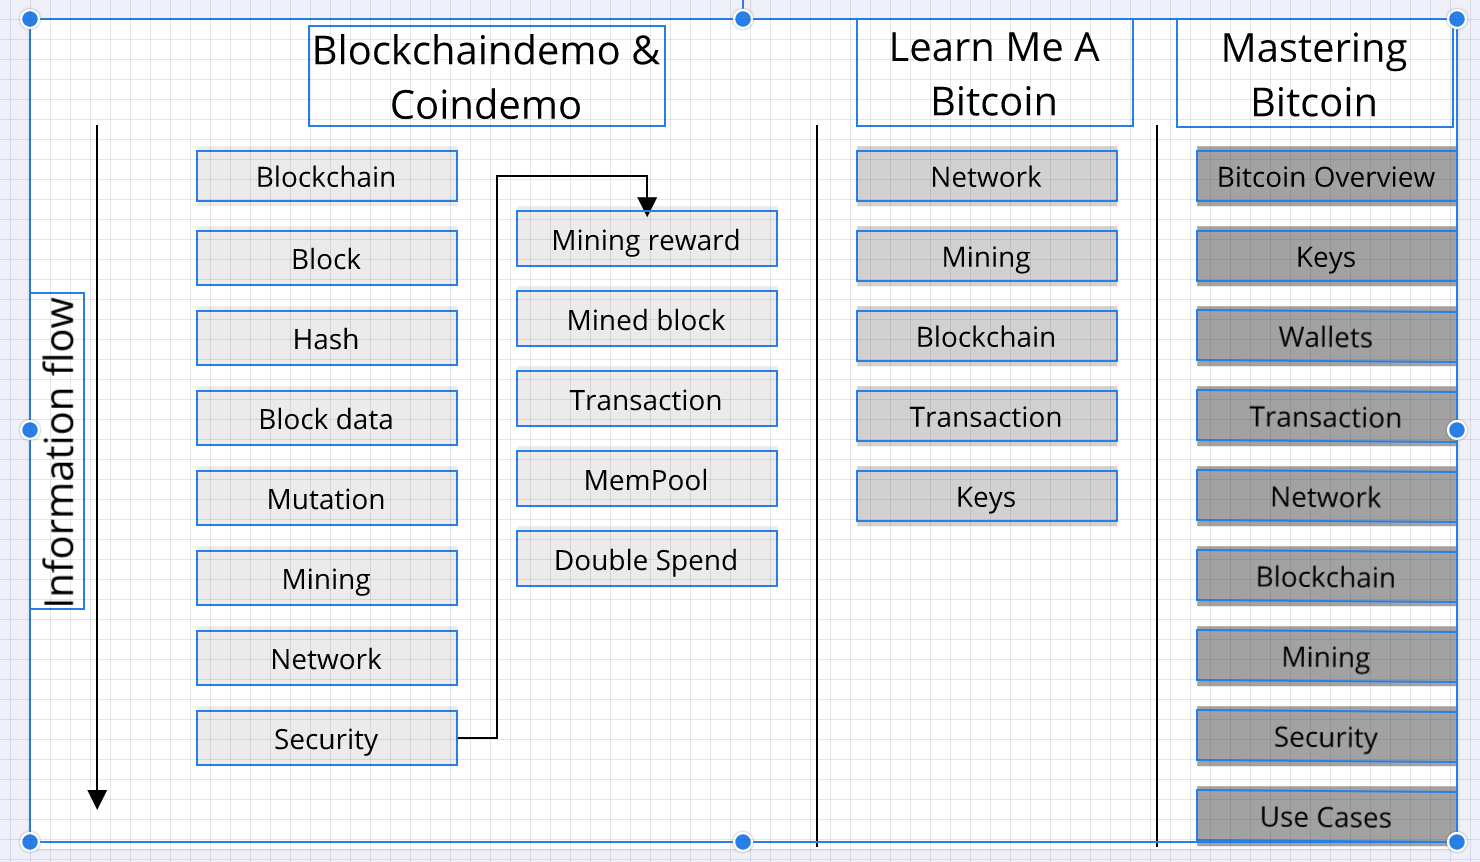
\includegraphics[width=\linewidth]{latex-vorlage_v1.5/graphics/ProcessBC.png}
    \includesvg[width=\textwidth]{graphics/BCExplanation}
    \caption{Comparison of the information flow from \textit{Blockchain}- and \textit{Coindemo}, \textit{Learn Me A Bitcoin} and \textit{Mastering Bitcoin}.}
    \label{fig:ProcessBC}
\end{figure}

The common terms and concepts that all of the presented projects define are: blockchain, mining, transactions, and the peer to peer network. Additionally, two of the three projects describe the role of cryptographic keys and blockchain's security features. However, none present these concepts in the same order as another, which suggests that the flow of information is less dependent on the technical concepts than on the author's choice and their way of storytelling. For this reason, a particular information flow of the more technical concepts cannot be derived from this comparison. However, it has become clear that the concepts and definitions of blockchain, mining, transactions, and peer to peer networking must be included. The artifact will hence discuss these concepts on a relatively high abstraction level during the first section (the guided tour). However, the user is given the possibility to learn about some of the concepts in more detail once the guided tour is finished. They will then be presented with an overview of the major elements of the blockchain technology which, when clicked upon, show additional information. 

\paragraph{Interactivity} As Mayer and other authors have stated, interactivity (if done correctly) provides a way to engage the audience in more meaningful learning.\footcites[Cf.][p.310]{MorenoInteractiveMultimodalLearning2007}[cf.][p.160]{ZhangInteractiveMultimediaBasedELearning2005}[cf.][p.190]{LeeScreenDesignGuidelines1999} The artifact will contain different elements (for navigating, controlling, and manipulating data) which motivate the audience to participate and play with the presented information. One of these elements is the presentation of how a cryptographic hash function works. The user will be able to enter a value and see the corresponding hash value. Similarly, the user will also be able to change the content of a block and see how such a change affects the appended blocks. Such interactions allow the user to explore the technologies actively and thus to learn more deeply. The full list of interactive elements is presented in \ref{sec:ArtifactDesign} as part of the design process. 

%as this interactivity is what is missing in most of the other existing explanations. For this purpose, the artifact will use different interactivity types (presented in \ref{sec:Interactivity}, such as controlling, navigating and manipulating. During the first part, the user interacts with the artifact as they follow the explanation by determining the speed of the presentation. The second part is more open to the user as it allows different concepts to be explored and these concepts will 

\paragraph{Visual information presentation} The findings from \ref{sec:Interactivity}, \ref{sec:GuidelinesMultimediaInstr}, \ref{sec:ExistingSolutions}, as well as from the expert interviews show that information should be presented in an easy-to-understand manner. One possible way to engage the audience in meaningful learning is to use visualizations of the information with which the audience may interact (multimedia principle and interactivity principle).\footcites[Cf.][]{RalphBeckmann_Interview}[cf.][p.1025]{DomagkInteractivitymultimedialearning2010}[cf.][p.311]{MorenoInteractiveMultimodalLearning2007}[cf.][p.290]{Betrancourtanimationinteractivityprinciples2005} For this reason, the artifact will contain different visualizations to support the explanation. One of these visualizations will present a decentralized network as opposed to a centralized network and another will present how the different blocks are linked with each other. Regarding the way of information presentation, note that the information will be provided in the form of written text. Although the modality principle suggests a different approach (presenting words as speech rather than on-screen text) to distribute the cognitive loads on different sensory channels, this principle is only partially applicable to the situation as the information contains a number of technical terms with which the audience is unfamiliar and which should therefore remain visible.\footcite[Cf.][chapter 6, paragraph 1]{ClarkElearningscienceinstruction2016} Additionally, as this artifact may be used for demonstrations during trade fairs or conferences, a solution with no audio files is preferred for the following reasons: simpler set-up, less equipment necessary, and the possibility to begin a conversation with the partner at any time. To conclude, the visualization's intent is to underline the presented information (in written form) and thus to make the information easier to understand. That is why the graphics used should be simple and pithy. Since graphics and visualizations in addition to text are a tool to foster meaningful learning (multimedia principle), they must be understood as such and hence should be used only in suitable situations. 

\section{Requirements specification} \label{sec:ReqSpec}
While the previous paragraphs have simply described some characteristics the artifact will have, this section formally defines the requirements the artifact will have to meet. A detailed specification (regarding content, structure, and design), which is based on theoretical principles and insights gained from literature reviews and expert interviews, allows for a well-structured and theory-led approach to the design and development phases of the artifact. Where applicable, an arrow ($\rightarrow$) is used to indicate which principles and insights provide the basis for a particular requirement.

\paragraph{Content} The artifact must present the following information: 
\begin{enumerate}[nosep]
\newcounter{foo}
    \item A short overview of cryptoeconomics. This includes the financial aspect (What is money and how does it work?), the IT aspect (What are distributed systems? How do they reach a shared state?), and the economics/business aspect (How does game theory apply to this situation and what is incentivization?) $\rightarrow$ \cite{RalphBeckmann_Interview} P86 and P122
    \item A description of a peer to peer network and the nodes within
    \item A blockchain definition 
    \item A differentiation between blockchain, distributed ledger technology and other concepts such as distributed file systems $\rightarrow$ \cite{DanielKaltenbach_Interview} P46 and \cite{RalphBeckmann_Interview} P111
    \item A description of blockchain's use cases $\rightarrow$ \cite{RalphBeckmann_Interview} P113, \cite{DanielKaltenbach_Interview} P14, P57 and \cite{BjoernPaulewicz_Interview} P70, P75
    \item A description of consensus mechanisms and mining methods (proof of work and proof of stake)
    \item A definition of transactions
    \item A definition of smart contracts
    \item A description of cryptographic hash functions
    \item A description of public and private key cryptography
    \item A description of block mutation effects
\setcounter{foo}{\value{enumi}}
\end{enumerate}

\paragraph{Graphical design} The artifact must be designed along the following specifications:
\begin{enumerate}[nosep]
\setcounter{enumi}{\value{foo}}
    \item The text is accompanied by explanatory visualizations $\rightarrow$ multimedia principle and contiguity principle
    \item The graphics are simple symbols and easily identified
    \item Important graphics are visually highlighted $\rightarrow$ cueing
    \item Animations are used to transition between different topics
    \item A uniform gamut of colors is used
    \item Only the relevant information is visible at one time $\rightarrow$ segmenting principle
    \item The overview uses symbols to present every concept
\setcounter{foo}{\value{enumi}}
\end{enumerate}

\paragraph{Structure} The artifact must present the content in the following manner:
\begin{enumerate}[nosep]
\setcounter{enumi}{\value{foo}}
    \item The user may choose to follow a guided tour or to skip it and view an overview of the concepts $\rightarrow$ guided discovery principle and individual differences principle
    \item The guided tour presents small text boxes which contain a description of one specific topic $\rightarrow$ segmenting principle and modality principle
    \item The user follows the tour by clicking through the different text boxes $\rightarrow$ interactivity principle
    \item The user may go back to a previous topic or quit the guided tour by using a site map $\rightarrow$ site map principle
    \item The guided tour serves as an introduction for the second part $\rightarrow$ pretraining principle
    \item The overview provides access to more detailed information on a certain topic $\rightarrow$ segmenting principle
    \item The overall language meets that of a novice audience and uses friendly, conversational style wording $\rightarrow$ personalization principle
    \item At the end of the guided tour, the user is directed to the second section: the overview
    \item The user can choose a topic of their interest from the overview for more detailed information $\rightarrow$ segmenting principle
    \item As part of the detailed information, some concepts allow interaction and manipulation of data $\rightarrow$ interactivity principle
    \begin{enumerate}
        \item The user can enter a value into a text field and is presented with the hashed value
        \item The user can create a pair of keys 
        \item The user can mutate a block and see the effects of that change on the blockchain
    \end{enumerate}
\setcounter{foo}{\value{enumi}}
\end{enumerate}

\paragraph{Technology} To ensure its usability and utility, the artifact must fulfill the following technical requirements:
\begin{enumerate}[nosep]
\setcounter{enumi}{\value{foo}}
    \item The solution is location independent, so that it can be presented in various settings
    \item The solution processes user interactions and user input and reacts accordingly
    \item The solution is easily adapted, e.g., to conform to new branding requirements or to include new information
\end{enumerate}


% \subsection{Dashboard content}
% \textit{What exactly should the dashboard visualize?}
% State the requirements that come from the requirements analysis

% \subsection{Technology for dashboard development}
% \begin{itemize}
%     \item What should the technology be able to do? What are the requirements? (Should come from the interviews)
%     \item What possible technologies are there to build a dashboard? 
%     \item Compare these techs with respect to the formulated requirements and choose a solution/combination(?)
% \end{itemize}
\chapter{Design and development}
Based on the requirements defined in the previous section, this chapter covers the design and the subsequent development of the solution. While the first section presents the preparatory steps leading to the final design of the artifact, the latter section presents the choices that are made regarding technology, development environment and implementation to transform the artifact from a simple design to a working solution.

\section{Designing the artifact} \label{sec:ArtifactDesign}
The first step of the design process consists of specifying the flow of the information. As discussed in \ref{sec:InformationPresentation}, there is no rigid, predefined way of introducing the different concepts to the audience, instead it is upon the author to lead the user through the explanation. The chosen approach divides the artifact into two parts: the guided tour and the overview. This division lets the user decide whether to follow the guided tour which presents a high level introduction to the different topics (and then leads to the overview) or whether to jump straight to the overview which presents these topics, too, but in a more detailed and interactive manner. The following paragraphs now deal with the guided tour before the structure of the overview is presented.

\paragraph{Guided tour} Taking into account the requirements from \ref{sec:ReqSpec}, figure \ref{fig:DesignConcept} presents the flow of information. %It is for this reason that the following graphic (figure \ref{fig:DesignConcept}) is developed which presents the flow of information.
While the number of boxes behind a topic indicates how much text there will be in the final design, any more detailed information is omitted and will be presented in an ensuing step. 

\begin{figure}
    \centering
    \includesvg[width=0.8\linewidth]{graphics/DesignConceptSteps.svg}
    \caption{Flow of the presented information during the guided tour}
    \label{fig:DesignConcept}
\end{figure}

Keeping in mind that the target audience has only little to no knowledge about blockchain technology, the information is presented within a narrative context. With the help of two fictional actors, Anna and Bob, the audience is presented with a brief summary of the finance aspect of cryptoeconomics. This includes a brief summary of the role of money, the role of banks, the process of transferring money between parties and finally how new technologies have affected the way money is accessed and distributed. After explaining how money is digitally transferred in traditional systems, the concept of distributed systems is introduced in form of multiple bank symbols representing a decentralized peer to peer transaction system. Nodes (participants in that network) and their different types are presented and it is shown how Anna and Bob would interact with that system instead of a centralized system. An important information is also the way the distributed system reaches a shared state as compared to a centralized system. By providing a concrete comparison between these two systems (centralized and distributed), the user should be able to recognize the difference more easily. After presenting the nodes, it must be made clear why the system should behave a certain way. As this is based on game theoretical concepts, these are introduced subsequently: By continuing the story line of Anna and Bob (what happens if Anna's node is malicious and wants to hurt the network?) it is shown that a node is incentivized to act in favour of the overall system as that is in its own interest. Once these three concepts, constituting the three pillars of cryptoeconomics, have been introduced, the concept of public and private key infrastructure is presented by showing how Anna and Bob both use their key pairs to create transactions in the network. The concept of transactions then guides the user to one of the technical key characteristics of blockchain: the blocks and the cryptographic hash functions that link those blocks to form an immutable chain of transactions. As indicated in figure \ref{fig:DesignConcept}, this part of the explanation is most likely to need the most text. This topic is then followed by the presentation of consensus mechanisms which are used to attain the same state for every node in the network. Note that this part of the explanation appends to the topic of distributed systems (one shared state) in a way that the presented consensus mechanisms are specific to blockchain, whereas other distributed systems use a different mechanism to reach their shared state. Finally, the guided tour leads to a presentation of different use cases that blockchain enables. The user will see a list of various use cases with which they may interact to learn more. These use cases should be as easy to understand as possible in order to facilitate meaningful learning and to support the user in addressing possible use cases (specific to their position) more precisely.

Albeit the segmenting principle states that different concepts should be presented independently of each other, uncoupling these closely intertwined concepts from each other would actually prove harmful to the learning experience because the user would miss the context in which the specific concept is situated. Therefore, since repetitions cannot be avoided completely, this thesis' intention is to limit them in such a way that the explanation is not repetitive but presents a well rounded and easy to understand explanation of this complex technology.

\paragraph{Overview} At the end of the guided tour, the user is presented with the overview, presented in figure \ref{fig:OverviewPic}, that allows deeper insights into specific concepts.
In this overview, the audience is free to decide about which of the concepts they want to learn more. They are also given the opportunity to test out the concepts, such as playing with hashed values or changing the content of a block within the existing blockchain (see requirement 28a-c).

\begin{figure}
    \centering
    \includesvg[width=0.8\linewidth]{graphics/Blockchain_Overview.svg}
    \caption{Preliminary sketch of the overview section}
    \label{fig:OverviewPic}
\end{figure}

After the flow of information is defined, a rough sketch of the different screens the user is led through is designed on paper. The rough draft serves as the basis for the development and it is used to ensure that the requirements are included in the artifact.\footnote{As the sketches cannot portray which technology is used and what graphical design decisions are made (requirements 12 - 14 and 29 to 31), the actual requirements specification should be regarded during the development process, too.} The development of the artifact is described in the following section.

\section{Developing the artifact}

As a first task, before the actual task of implementing the artifact may begin, a technology needs to be identified that meets the requirements 29 to 31. The solution should be location independent, process user interactions and should be easily adapted by other developers in order to be applied in different situations.\footnote{This means that the different use cases presented in the overview may be changed to accommodate for a specific industry.} A possible solution is that of a web application due to its wide spread use, easy portability, easy deployment and the fact that changes may be easily implemented as the programming/scripting languages HTML, CSS and JavaScript are a common skill set among web developers. When following this approach, (regardless of whether the files are on a local machine or the web site is hosted online) the artifact is accessed via the browser allowing a quick set-up. This approach additionally allows the artifact's presentation from a remote location, if needed.

A first prototype of the artifact is developed within the web-based editor WebFlow. The editor allows the visual manipulation of code and changes to the CSS are reflected in real-time in the web preview of the editor). With this feature, the general style of the artifact's elements is quickly defined. The first prototype consists of a pop-up window which includes paragraphs of text and a button, as illustrated in figure \ref{fig:proto1}. WebFlow also allows to create simple interactions, so when the user hovers over the button or clicks it, the button gives visual feedback (changes in shadow style and upwards movement).

\begin{figure}
    \centering
    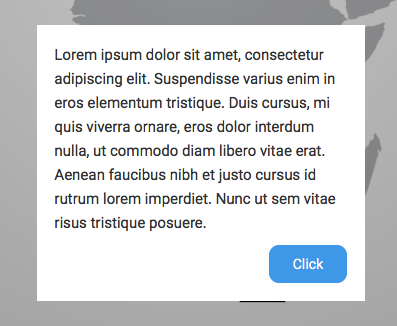
\includegraphics[width=0.4\textwidth]{latex-vorlage_v1.5/graphics/Prototype1.png}
    \caption{Prototypical pop-up window, styled in WebFlow}
    \label{fig:proto1}
\end{figure}

During the prototyping in WebFlow and the ensuing development of the artifact in the text editor Atom, the design considerations in form of the paper sketches and the requirements specification are continuously taken into consideration so that the final artifact presents a complete instantiation of the defined solution space.

The landing page (index.html) of the web page consists of two simple buttons which redirect either to the guided tour (guided-tour.html) or the overview (overview.html) (as illustrated in figure \ref{fig:ButtonStyle}, corresponding to requirement 19). In order to ensure consistent style, all pages access a shared CSS file and classes are defined to which the elements are assigned (such as the buttons of \texttt{class = "ButtonsMain"}).  

\begin{figure}
    \centering
    \includesvg[width=\textwidth]{graphics/protoAll.svg}
    \caption{Buttons, styled by \texttt{.ButtonsMain}, on the landing page redirect to either the tutorial or the overview}
    \label{fig:ButtonStyle}
\end{figure}

\paragraph{The guided tour} Once the user has clicked on the button \textit{Let's start the tour}, they view a short intro to the guided tour, stating its purpose and informing the user that the tour continues by clicking on the button on the bottom right of the ensuing pop-up windows (requirement 21). The purpose of this short introduction, written in a thoughtful and friendly manner (corresponding to requirement 25), is to support the user's curiosity, making them more interested in and receptive to the following explanations. Corresponding to the requirements 12-15 and 20, the user is first presented with an explanatory paragraph and the included information is then represented by a simple animation. These animations will be described in more detail in the following paragraphs while the order of the different concepts corresponds to the information flow of figure \ref{fig:DesignConcept}. The exact wording of these explanations will also not be explained in further detail but may generally be described as a high-level summary of chapter \ref{chap:Blockchain}, presented in more layman terms.

The tutorial begins with the presentation of the two actors Anna and Bob who accompany the user throughout the tutorial. Figure \ref{fig:Animationline} illustrates the animations in the first part of the tutorial which deals with the financial aspect of cryptoeconomics (requirement 1) and shows how money may be transferred between parties. The dashed arrows and lightly transparent symbols are added to the screen clippings for additional clarity. Firstly, the two actors are introduced (a), then Anna sends Bob money in form of cash which he receives directly (\ref{fig:Animationline}b). In \ref{fig:Animationline}c, Anna has deposited her capital with a bank which she then orders to transfer money from her account to Bob's. As indicated in the figure, the bank now serves as an intermediary, keeping a small share of the transaction for its service. After this, the user is introduced to the concept of distributed systems (requirement 2), as Anna transfers money to Bob where numerous nodes in the network process the transaction. It is made clear to the user that all nodes must have the same view of the system to ensure the validity of all transactions. The tutorial continues by explaining how the participating nodes are motivated to participate in favor of the network and how Anna publishes a transaction (requirement 7) by signing it with her private key.

\begin{figure}
    \centering
      \includesvg[width=\textwidth]{graphics/Animations2.svg} 
    \caption{Animations about cryptoeconomics: a) Anna and Bob; b) Anna gives money to Bob directly; c) Anna transfers money to Bob via a bank; d) Anna transfers money to Bob via a distributed system}
    %\caption{Summary of animations inside the guided tour}
    \label{fig:Animationline}
\end{figure}


\begin{figure}
    \centering
      \includesvg[width=\textwidth]{graphics/Animations3Block.svg} 
    \caption{Animating the inclusion of transactions in a block}
    \label{fig:AnimationBlock}
\end{figure}

The tutorial then proceeds with an illustration of how transactions are added to a block, what other data these blocks contain and how they are linked to each other (requirement 3). Figure \ref{fig:AnimationBlock} shows how the transactions are added one after the other inside a container indicating the sender, recipient and amount. Once the container is filled, a pop-up window lists and explains the other data points of a block (time stamp, block number, current and previous block hashes) before the container is enclosed by a block containing these data points. When clicked on the button beneath the block, a text box opens in its place leading to the topic of consensus mechanisms. For this, the block is minimized and an animation illustrates the block's propagation throughout the network and its addition to the each node's local version of the blockchain.

Thereafter, the user is led to the final part of the guided tour which presents a summary of different use cases that the blockchain technology enables (requirement 5 and 8). The three different categories of use cases (transactions of value, proof of existence, and automation and machine payments) are situated at the bottom of the page and indicate that they contain more information by slightly changing their style when the user hovers over it (same changes as for the buttons). If clicked upon, the specific element expands to uncover further information and detailed examples of these use cases. Figure \ref{fig:AnimUC} shows the different states: The left element (status:hover) is positioned slightly higher and has a different box shadow (altogether simulating an upwards 3D-movement) than the other elements. While the right element shows no change in style (status:none), the center element is expanded because the user has clicked on it, thus executing a JavaScript function which adds or removes the class \texttt{.expanded} from the element's class list accordingly. The more practical example is presented in two parts: The situation (or problem) and the purpose (argument why blockchain solves this problem). By presenting this example in this simple manner, the user may quickly understand in which situations the blockchain technology might be useful and transfer the information from this concrete example to their own field of expertise. Once the user has finished reading through the different use cases, they may go to the overview by clicking on an arrow in the top right stating \textit{Go to the overview} which redirects to \texttt{/overview.html} (requirement 23 and 26). 

\begin{figure}
    \centering
    \includesvg[width=\linewidth]{graphics/AnimationUseCases.svg}
    \caption{The different states of the use case elements}
    \label{fig:AnimUC}
\end{figure}


\paragraph{The overview}
The overview may be considered a natural extension of the guided tour as it offers more detailed information regarding consensus mechanisms, transactions, private and public key cryptography and hash functions. As can be seen in figure \ref{fig:AniOW}, the overview page is of identical layout as the other pages in the guided tour, but additionally includes a hexagon-shaped element in the center of the distributed system (requirement 18). This element, as well as the icons of Anna and Bob and the up-most block on the blockchain on the right-hand side of the page provide the entry points for further explanations. The overview therefore serves as the centre from which all information may be accessed (requirements 17, 24, and 27).\footnote{There is also a link in the top right corner redirecting to the beginning of the guided tour, should the user have skipped it by accident.} To inform the user of these entry points, the elements change their style when the user hovers over them (requirement 14). The change of style is similar to that of the use case elements, described earlier in this chapter. However, the elements also reveal tool tips which intend to motivate the user to click on these elements. For example, the tool tips on the icons of Bob and Anna state \enquote{Learn more about how participants can send transactions} and redirect to the page \texttt{/transactions.html}. This page explains how the user can create their own public and private key pair which they would need in order to execute a transaction (requirement 10). The second element that offers more information about a shortly presented topic is the hexagon in the center of the page. It leads the user to the page \texttt{/consensus.html} and firstly explains the general role of consensus mechanisms for blockchain technology (requirement 6) and then lists five of the most often implemented consensus mechanisms (proof of work, proof of stake, leased proof of stake, delegated proof of stake, and proof of burn). Since proof of work and proof of stake are the most well known mechanisms, they are represented by a respective icon (pick axe and vault). All five elements may be expanded individually to reveal more detailed information about the respective mining techniques, if the user wants to know more about these consensus mechanisms. The third element, the newest block in the blockchain, motivates the user to \enquote{learn more about hash functions} as it redirects to the web page \texttt{/hashes.html} (requirement 9). There, the nature and function of hash functions is explained in more detail. It is also explained how a change in a previous block affects its hash value resulting in invalidating all ensuing blocks as they refer to each other by these hashes. This effect is also called block mutation effect (requirement 11). However, this site also allows the user to play with these hash functions. They are presented with a text area into which they are instructed to write any arbitrary value (requirement 28). With a click on the button in the center, the input is hashed and presented in the output text area as well as in the element at the bottom which shows the overall history of this session's entered values and corresponding hashes. The history element provides two preset values (\enquote{Hello World} and \enquote{hello world}) which show that even almost identical values result in significantly different hashes. The presented hash values are results of the SHA-256 (Secure Hash Algorithm returning a value of 256 bits) function which is used by the bitcoin implementation. This version is written in JavaScript and takes any ASCII value which it then converts to a SHA-256 hash.\footcite[][]{LuffJavaScriptSHA256demo2014}

\begin{figure}
    \centering
    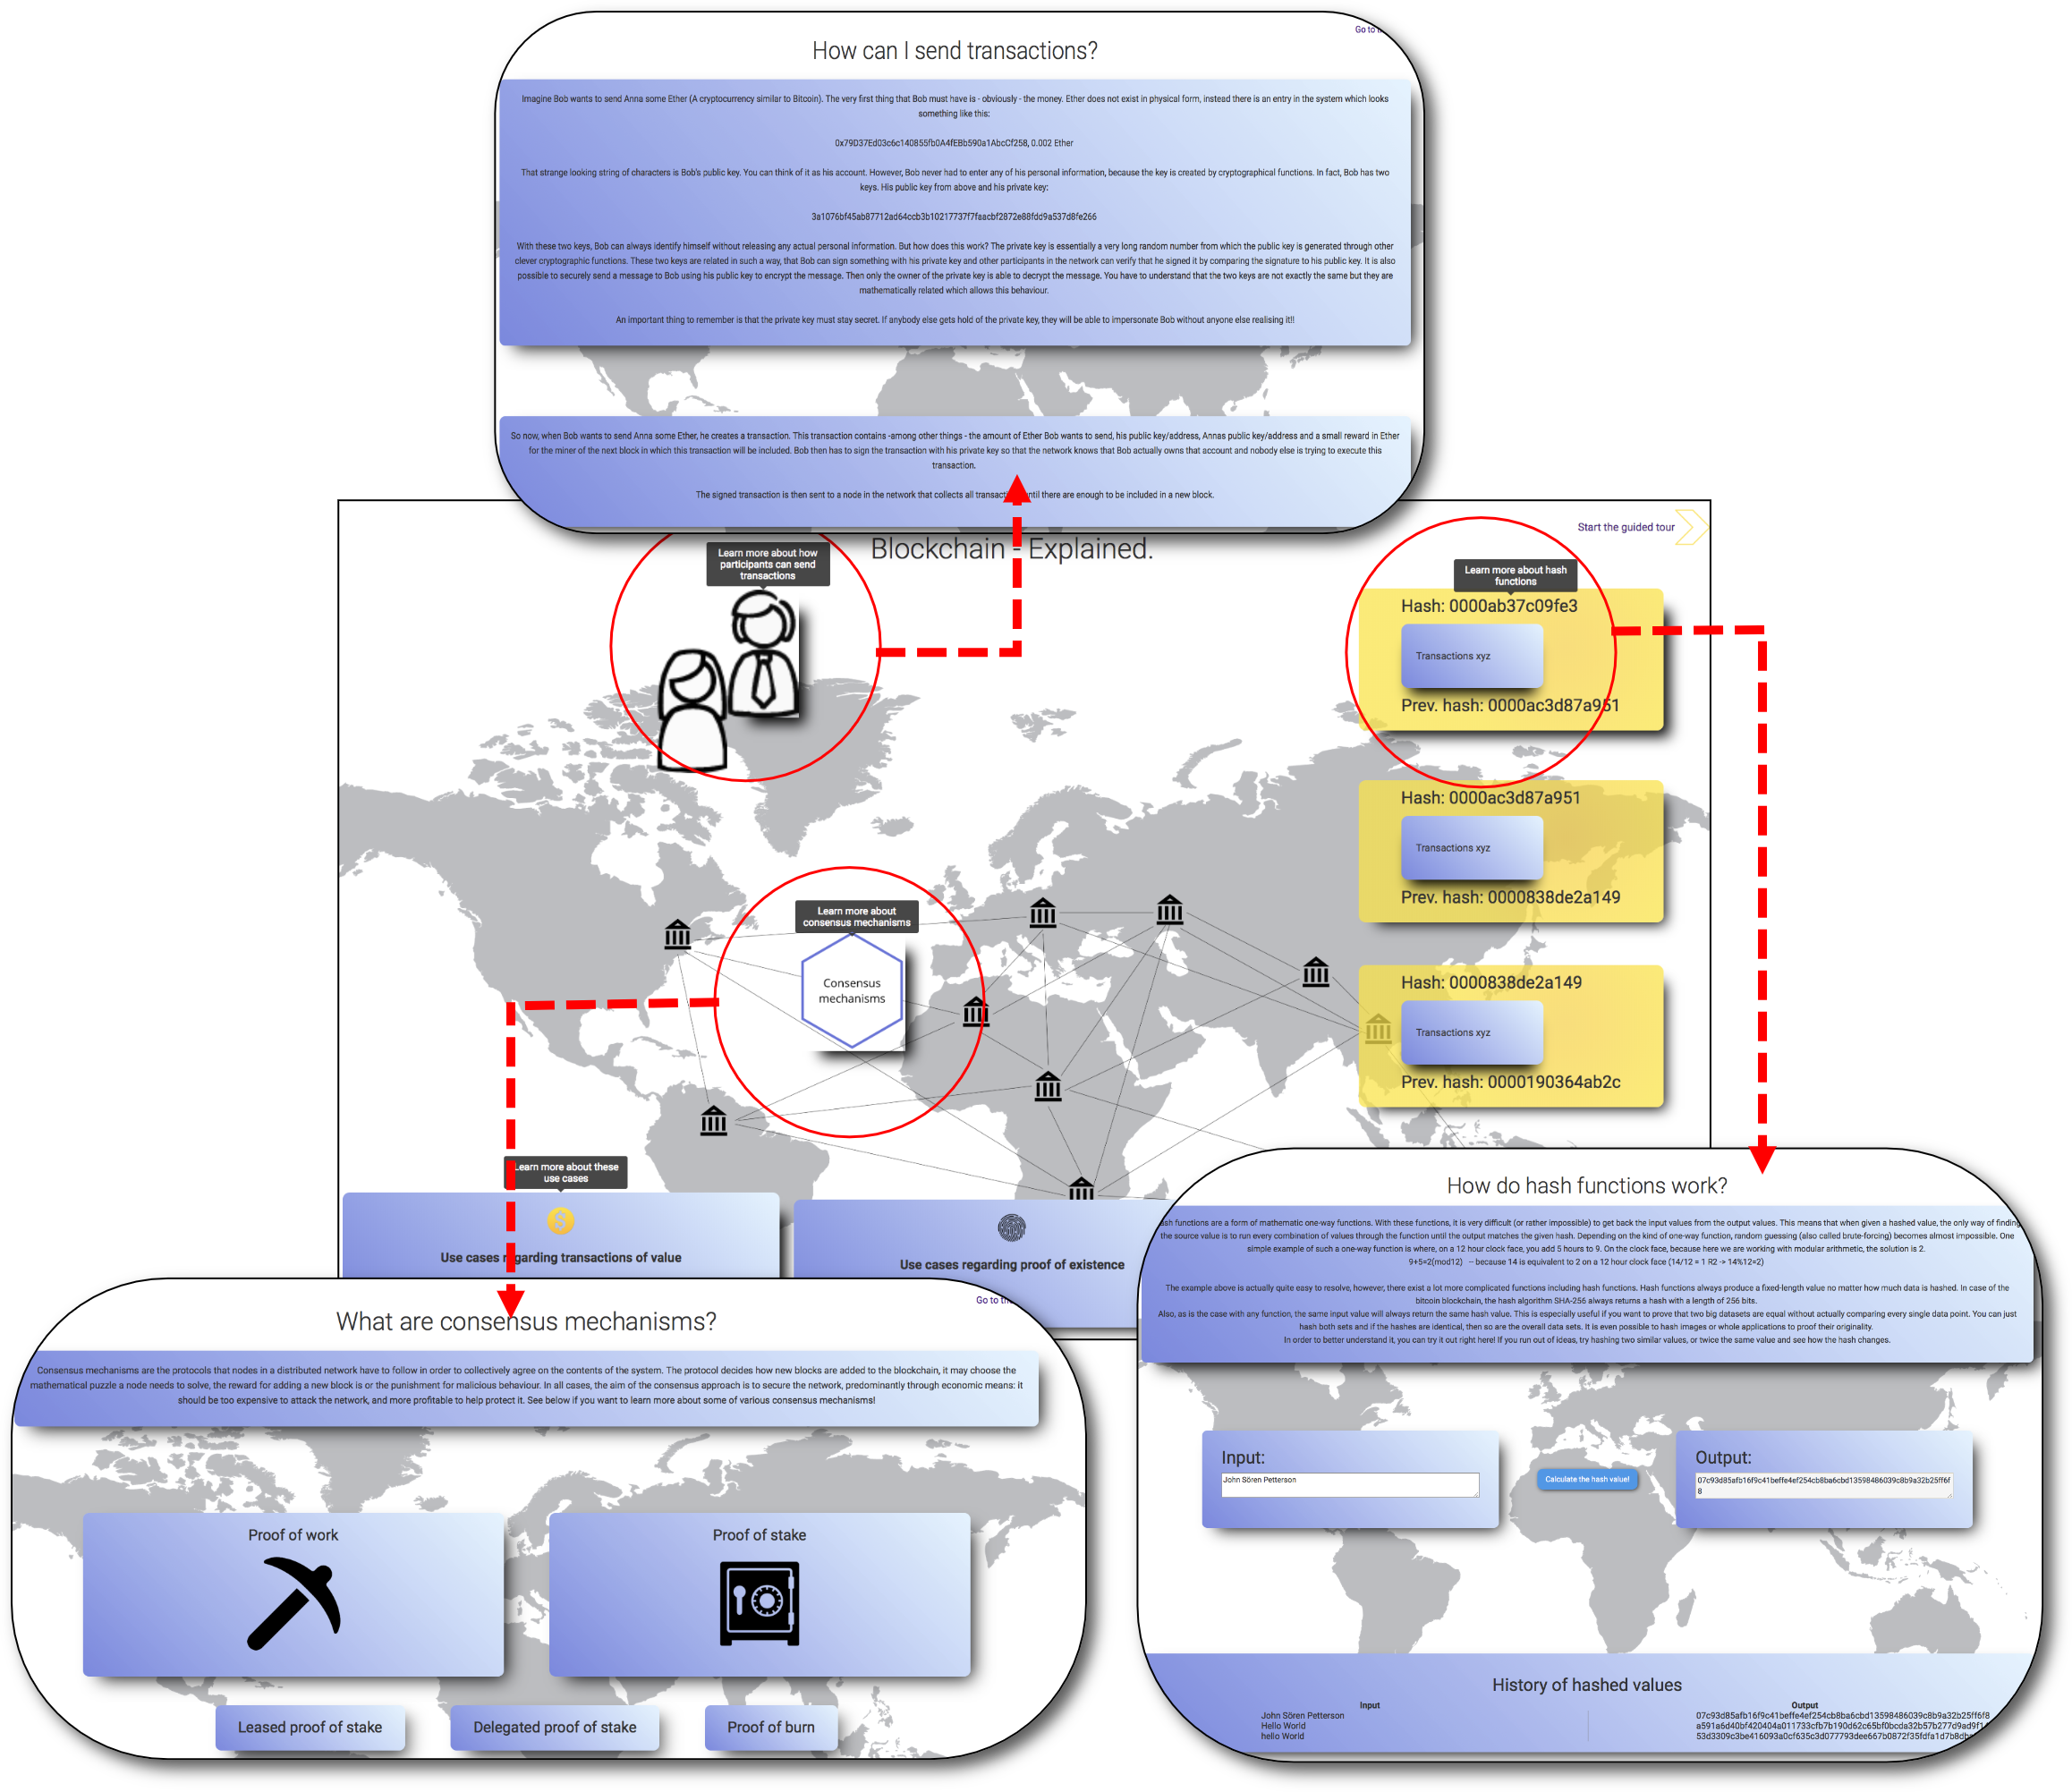
\includegraphics[width=\textwidth]{latex-vorlage_v1.5/graphics/overview.png}
    \caption{The symbols within the overview lead to more information regarding transactions, consensus mechanisms, hash functions and use cases}
    \label{fig:AniOW}
\end{figure}

Regarding the requirement of consistent styling (requirement 16), all pages have the same background, consistent font styles, same palette of colour (grey for background and texts, gradient blue for large-area elements and yellow highlights) and a link in the right top corner which either leads to the tutorial (from the overview page) or to the overview (from all other pages). In addition, similar elements (e.g. the buttons or the blue containers) are assigned the same classes so that a change in styling affects all elements equally. Hover effects as well as on-click-expansion and the revealing of hidden information are also defined in the CSS file.\footnote{A JavaScript function, called by \texttt{onclick="expand('id')"}, handles the logic of assessing whether a class should be added or removed from the element's class list.} 


Unfortunately, due to constraints in time and resources, it has not been possible to implement more interactive elements similar to that of the hash function (see requirements 28b and c), although the thesis suggests that especially these opportunities to interact with the information allow for meaningful learning to occur. However, the evaluation, described in the following chapter, shall assess how helpful this feature is to the learning experience. If positive, the disregarded features might be included in the next iteration of the artifact. 
\chapter{Implementation and Evaluation}

This chapter will evaluate the artifact. First, the artifact's feasibility is demonstrated by utilizing it as an alternative to existing learning resources for new students at the \enquote{StudyLab} team. This demonstration is then extended to serve as the basis for a rigorous naturalistic evaluation which assesses the most relevant properties of the evaluand. The results are presented and discussed. Finally, on the basis of the discussion's insight, possible improvements to the artifact are presented.

\section{Exemplary demonstration: Onboarding new students to the blockchain team} \label{sec:demo}

Once the artifact is developed, a suitable context needs to be identified in which the artifact may be implemented and demonstrated. As the artifact's purpose is to give a short overview of the blockchain technology and its use cases to people who are yet unfamiliar with this technology, the context must present an environment that is applicable to the problem space. Possible situations may be: informal client meetings, seminars, various fairs, or the onboarding of new employees. This paper suggests that the artifact may be utilized in any of these situations.

The demonstration serves as a light-weight evaluation to prove the artifact's feasibility, i.e. that the artifact solves one instantiation of the formulated problem. In this case, the instantiation of the problem is that of the onboarding process of corporate students to the enterprise's \enquote{StudyLab} department which works on blockchain related projects. Contrary to recent hires, corporate students are already familiar with the organization's culture, structure, communication, and tools. Therefore, the onboarding process does not focus on introducing these students to the organization, it solely focuses on introducing them to the blockchain technology and its use cases. Generally, the students are given access to a \enquote{Student Learning Guide} which is a collection of various blockchain learning resources, including $\geq$ 60 hours of video material, numerous introductory articles as well as various technical resources regarding specific blockchain implementations. Although the learning guide is extensive, working through the resources is time intensive and novices appear to have problems gaining an initial high-level understanding because they focus on technical details too early.\footcites[Cf.][]{RalphB_Interview} This situation therefore offers an appropriate opportunity to assess the artifact's feasibility.

Since the artifact is a web page, it is quickly deployed and may be accessed from within the organization's intranet. New students joining the \enquote{StudyLab} team are given the link to the artifact (also referred to as tutorial) and are asked to go through it. Because no other appropriate situations were available for a more thorough evaluation at that point of time, and because the described problem context is considered excellently suited to prove not only the artifact's feasibility but also its quality and effectiveness. The demonstration of the artifact is extended to also serve as evaluation. The next section describes the evaluation method therefore in more detail.

%The demonstration is done for new students that are going to work in the department of StudyLab which treats the blockchain technology. 

\section{Evaluation} \label{sec:Evaluation}

The exemplary demonstration lends itself excellently for a more thorough evaluation of the created artifact. As stated by \cite{HevnerDesignScienceResearch2004} and agreed upon by the design science research community, such evaluation plays a \enquote{crucial} role in design science research.\footcites[Cf.][p.258]{MarchDesignnaturalscience1995}[Cf. in addition][]{PfeffersDesignScienceResearch2007}{HevnerDesignScienceResearch2004}{Pries-HejeComprehensiveFrameworkEvaluation2012}{Pries-HejeStrategiesDesignScience} A rigorous evaluation of the artifact and its qualities must take place in order to provide evidence that the artifact achieves its purpose, i.e. that it solves the identified problem. \footcites[Cf.][p.425]{Pries-HejeComprehensiveFrameworkEvaluation2012} The evaluation should furthermore also assess how well the artifact solves the problem. This is done by first identifying the relevant evaluation criteria. These may include - in addition to the in guideline 3 \textit{Design Evaluation} described properties of a design artifact (utility, quality, and efficacy) - properties such as Checkland and Scholes five E's (efficiency, effectiveness, efficacy, ethicality, elegance) or the artifact's purposefulness and implementability.\footcites[Cf.][p.427]{Pries-HejeComprehensiveFrameworkEvaluation2012}[cf. in addition][]{ChecklandSoftSystemsMethodology1990}
% Overall, the candidates of evaluation criteria should be chosen in such a way that they adequately identify the relevant strengths and short comings of the artifact so that its utility may be adequately assessed. At first, focusing on certain criteria and disregarding others may appear to inhibit a rigorous approach that is necessary to ensure the scientific nature of the artifact. But this selection of important criteria in fact ensures something of similar interest, the relevance of the applied methods with regard to the overall relevance of the design science research.\footnote{For more information about the interplay of relevance and rigor in design science research, see \ref{topic:relevance cycle}}

% While it is important to rigorously conduct the relevant evaluation methods in order to ensure the scientific nature of the design science research, In other words, even though rigorous evaluation methods must be executed to ensure the design science process is of scientific nature, the evaluation should nonetheless focus on the important properties in order to remain relevant.

Numerous different evaluation methods exist, ranging from observational, analytical, and descriptive to experimental, and testing methods such as illustrative scenarios, technical experiments, case studies, or action research.\footcites[Cf.][p.86]{HevnerDesignScienceResearch2004}[cf.][p.4 et seq]{PfeffersDesignScienceResearch2012}
%Yet, these do not represent the entire list of relevant evaluation methods available to design science researchers. As \cite{PfeffersDesignScienceResearch2012} found out, the majority of researchers conduct technical experiments, followed by illustrative scenarios and case studies. However, the method chosen depends largely on the type of artifact and its qualities to be evaluated. In the case of information systems research, more qualitative approaches such as case studies or subject-based experiments are pursued as these are deemed more relevant.\footcites

The following paragraphs present the evaluation method that is chosen on the basis of Pries-Heje/Baskerville/Venable's evaluation strategy framework before results of that evaluation are illustrated and subsequently discussed. 
%validity, utility, quality, efficacy; Purposeful? and implementability?

\subsection{Method} \label{subsec:EvaluationMethod}

While Hevner et al. have identified a number of different evaluation methods, they have not offered any guidance on the choice of appropriate evaluation strategies. It is for this reason that Pries-Heje et al. have proposed a framework for evaluation in design science research which constitutes the scientific basis of this evaluation process.\footcites[Cf.][p.11 et seq]{Pries-HejeComprehensiveFrameworkEvaluation2012} The framework presents a matrix that compares artificial and naturalistic evaluation methods with ex ante and ex post evaluation methods. The authors also suggest a four-step approach which (1) analyzes the requirements for the evaluation to be designed, (2) connects these requirements to the dimensions in the matrix, (3) selects the appropriate evaluation method that aligns with the chosen strategy quadrants in the matrix and (4) then conducts the evaluation.\footcites[Cf.][p.13]{Pries-HejeComprehensiveFrameworkEvaluation2012} 

\paragraph{Method selection} Corresponding to the first step, the requirements for the evaluation context are defined. As the evaluand is the developed instantiation of the artifact, the design process is out of the scope for this evaluation (it will however be critically reviewed in \ref{sec:Reflection}) The evaluation must assess the utility, efficacy, efficiency, purposefulness and implementability, but ethicality and elegance may be disregarded as, considering the constraints of time, cost and resources, they do not help directly identify how well the instantiation solves the problem. Since the problem statement also infers that existing explanations of the blockchain are insufficient, the evaluation must also compare the developed artifact against existing explanations. Taking these requirements into consideration, a naturalistic ex post (after artifact construction) evaluation method is deemed the most fitting. Naturalistic evaluations evaluate the artifact in its real environment and even though they are more costly to perform and may suffer from misinterpretation or confounding variables, a naturalistic approach is considered to be the \enquote{real proof of the pudding}.\footcites[Cf.][p.6, p.3 et seq]{Pries-HejeStrategiesDesignScience}[cf.][p.80]{PfeffersDesignScienceResearch2012} Once an appropriate strategy is selected, the third step is concluded by deciding on the best fitting evaluation method. Possible methods, among others, are action research, case studies, participant observation and surveys, of which the latter two are considered most appropriate for this evaluation as they allow real users to test the artifact in a real environment and the evaluation data (whether quantitative or qualitative) is collected by the surveys in form of questionnaires.  

\paragraph{Materials} The material for the evaluation comprises a questionnaire as well as the evaluand (the artifact) and the two most relevant YouTube videos (\href{https://www.youtube.com/watch?v=r43LhSUUGTQ}{Understand the Blockchain in Two Minutes by the Institute for the Future} and \href{https://www.youtube.com/watch?v=SSo_EIwHSd4}{How does a blockchain work by Simply Explained Savjee}) as comparison. The videos, previously identified during the requirements gathering phase, are well suited as comparison as they cover the same concepts as presented in the artifact but lack its interactivity. The questionnaire is divided into two sections because the first part is to be answered before viewing the artifact or the videos and the other part is to be answered afterwards so that it is possible to identify the changes in understanding caused by the explanations. The questionnaire is included in the appendix \ref{anhang:EvaluationQuestionnaire}. 

\paragraph{Participants and procedure}
For this evaluation, 22 students (16 male, 6 female) from the HPE Dualstudy program are asked to participate. While the sample size is relatively small and not representative, this convenience sample should be sufficient to collect a variety of opinions which allow an assessment of the artifacts qualities. The participants are given a brief description of the overall project and the purpose of the evaluation before asked to fill in the first part of the questionnaire. The division of the questionnaire serves two purposes: 1) It includes the questions defined in \ref{fig:TargetGroup} to identify the participants that match the target group and 2) some questions are asked both before and after the participants learn about blockchain in order to assess if their growth of understanding. Of the 20 participants, four fall outside of the target group and are thus excluded from the process. The remaining 16 participants are then grouped in two groups on the basis of their given answers to question 2 (their perceived understanding of blockchain) so that both sets remain comparable.\footnote{The division is executed manually by comparing the two highest values and putting the respective participants in separate groups. If both values are equal, then the next two values are compared in the same way. This is continued until there are either no more participants to be grouped (example: six participants with the levels of 6, 6, 4, 4, 1, 1.) or until the two highest values are not equal. Then the participant with the highest value is put in the first and the latter in the second group. To counterbalance this, should such a case occur again, the participant with the higher value is then put in the second group and vice versa. This is continued until all participants are assigned to a group.}
They are then given access to the second part of the questionnaire as well as the videos (group 1) or the tutorial (group 2). If during this process any questions appear, the researcher is available to respond to the participants' questions. They are asked to view the resources, to respond to the remaining questions directly afterwards and to send their responses via email to the researcher which are summarized in the following section.

\subsection{Results} \label{subsec:EvaluationResults}

To put the artifact's qualities to a test, the evaluation focuses on the question whether and how well the artifact achieves its goal of explaining blockchain technology to a novice audience compared to existing resources such as YouTube videos. It is for this reason that the questionnaire is divided in two sections containing redundant questions (among others) hence not only allowing a comparison of the two different groups (videos and tutorial) but also their learning progress (a priori and a posteriori).

\paragraph{Questions 1 and 5}The first questions 1(a-e) establish that the participants fit the target group. The participants are confronted with the questions again (5 (a-e)) after having reviewed their respective resources in order to determine whether they have gained enough understanding to no longer be considered \enquote{novices}. The results are presented in the following figure. 

As illustrated by figures \ref{fig:ResultsVideos} and \ref{fig:ResultsTutorial}, the a priori responses show that almost all participants have heard of bitcoin (17 of 18) and of blockchain (15 of 18), but fewer feel they understand bitcoin (10 of 18) or blockchain (9 of 18). Contrary to these results, one participant responds positively to the final question of this set (\enquote{Do you know what cryptoeconomics means?}) while the others - of which eight have responded exclusively positively to the previous questions - negate the final question.

\begin{figure}[htbp]
    \centering
    \begin{tabular}{l r}
            \begin{tikzpicture}
	        \begin{axis}[name=plot1,
	            xbar stacked,
            	bar width=15pt,
                enlargelimits=0.15,
                legend style={at={(0.5,-0.20)},
                  anchor=north,legend columns=-1},
                xlabel={\# participants},
                xmin=0,
                xmax=9,
                symbolic y coords={1e, 1d, 1c, 1b, 1a},
                ytick=data,
                nodes near coords,
            	]
        	\addplot coordinates
        		{(1,1e) (4,1d) (7,1c) (5,1b) (9,1a)};
        	\addplot coordinates
        		{(8,1e) (5,1d) (2,1c) (4,1b) (0,1a)};
        	\legend{\strut yes, \strut no}
        	\end{axis}
            \end{tikzpicture}
            % \caption{Distribution of the \enquote{a priori} answers of group 2 (artifact)}
        & 
            \begin{tikzpicture}
	        \begin{axis}[
	            xbar stacked,
	            nodes near coords,
            	bar width=15pt,
                enlargelimits=0.15,
                legend style={at={(0.5,-0.20)},
                  anchor=north,legend columns=-1},
                xlabel={\# participants},
                symbolic y coords={5e, 5d, 5c, 5b, 5a},
                xmin= 0,
                xmax=9,
                ytick=data,
            	]
        	\addplot coordinates
        		{(2,5e) (9,5d) (9,5c) (7,5b) (9,5a)};
        	\addplot coordinates
        		{(7,5e) (0,5d) (0,5c) (2,5b) (0,5a)};
        	\legend{\strut yes, \strut no}
        	\end{axis}
            \end{tikzpicture}
            % \caption{Distribution of the \enquote{a posteriori} answers of group 2 (artifact)}
        \\
    \end{tabular}
    \caption{Distribution of the \enquote{a priori} (Q1) and \enquote{a posteriori} (Q5) answers of group 1 (videos)}
    \label{fig:ResultsVideos}
\end{figure}

\begin{figure}[htbp]
    \centering
    \begin{tabular}{l r}
            \begin{tikzpicture}
	        \begin{axis}[name=plot1,
	            xbar stacked,
            	bar width=15pt,
                enlargelimits=0.15,
                % legend style={at={(0.5,-0.20)},
                %   anchor=north,legend columns=-1},
                xlabel={\# participants},
                xmin=0,
                xmax=9,
                symbolic y coords={1e, 1d, 1c, 1b, 1a},
                ytick=data,
                nodes near coords,
            	]
        	\addplot coordinates
        		{(0,1e) (5,1d) (8,1c) (5,1b) (8,1a)};
        	\addplot coordinates
        		{(9,1e) (4,1d) (1,1c) (4,1b) (1,1a)};
        	% \legend{\strut yes, \strut no}
        	\end{axis}
            \end{tikzpicture}
            % \caption{Distribution of the \enquote{a priori} answers of group 2 (artifact)}
        & 
            \begin{tikzpicture}
	        \begin{axis}[
	            xbar stacked,
	            nodes near coords,
            	bar width=15pt,
                enlargelimits=0.15,
                % empty legend,
                % legend style={at={(0.5,-0.20)},
                %   anchor=north,legend columns=-1},
                xlabel={\# participants},
                symbolic y coords={5e, 5d, 5c, 5b, 5a},
                xmin= 0,
                xmax=9,
                ytick=data,
            	]
        	\addplot coordinates
        		{(6,5e) (9,5d) (9,5c) (8,5b) (8,5a)};
        	\addplot coordinates
        		{(3,5e) (0,5d) (0,5c) (1,5b) (1,5a)};
        	%\legend{\strut yes, \strut no}
        	\end{axis}
            \end{tikzpicture}
            % \caption{Distribution of the \enquote{a posteriori} answers of group 2 (artifact)}
        \\
    \end{tabular}
    \caption{Distribution of the \enquote{a priori} (Q1) and \enquote{a posteriori} (Q5) answers of group 2 (artifact)}
    \label{fig:ResultsTutorial}
\end{figure}

When presented with these questions for the second time, the participants answer more questions positively. While there is no change in responses for question 1a (18 of 19), the overall number of positive responses has risen significantly (+48\%). All participants state they know and understand blockchain technology and the final question also records a growth from 1 to 8 positive responses.

While there is no visible difference between the two different groups a priori\footnote{As should be expected \& hoped for, since the two groups should be comparable for the evaluation}, however focusing on the responses a posteriori, in group 1, a significant lower number responds positively to the final question. 7 participants of group 1 state they do not know what cryptoeconomics means whereas in group 2 only 3 participants voice that opinion. Furthermore, a total number of 7 participants answer all questions in the affirmative, thus no longer falling into the target group. Of these 7, 5 participants are part of group 2 (70\%).

\paragraph{Questions 2 \& 6} Tables \ref{tab:EvalResultsYesNoVIDEO} and \ref{tab:EvalResultsYesNoTUTORIAL} show the respective answers of group 1 (videos) and group 2 (artifact) to the question \enquote{[...] how confident do you feel about your knowledge about blockchain technology?}.
It is apparent from these tables that 78\% (14 out of 18 participants) feel more confident about their blockchain knowledge. However, there is significant difference between the two different groups and the distance between both values depending on the initial (a priori) value. Firstly, the confidence level of group 1 has in average increased by 0.89 points while that of the latter group has increased by 1.67 (an increase of 100\% compared to group 1). Secondly, the increase is higher for participants that stated a lower (< 4) level than those who stated a higher level initially. In fact, participants K1.1 (level 7), K1.6 (level 8), and K2.6 (level 9) have not stated any change, while participants of lower levels estimated an increase of (in average) 1.9 points (ranging from 1 to 3).   


\begin{table}[]
    \centering
    \begin{tabular}{l | l l l l l l l l l }
          Self-assessment & K1.1 & K1.2 & K1.3 & K1.4 & K1.5 & K1.6 & K1.7 & K1.8 & K1.9  \\
         \hline
         A priori (Q2) & 7 & 3 & 4 & 5 & 1 & 8 & 1 & 3 & 1 \\
         A posteriori (Q6) & 7 & 5 & 4 & 6 & 2 & 8 & 3 & 4 & 2 \\
          \hline 
         Difference ($\Delta_{2,6}$) & 0 & 2 & 0 & 1 & 1 & 0 & 2 & 1 & 1 \\
         Average & & & & & & & & & \textbf{0.89} \cellcolor[gray]{0.9} \\
    \end{tabular}
    \caption{Results of the self-assessment of group 1 before and after watching the resources}
    \label{tab:EvalResultsYesNoVIDEO}
\end{table}

\begin{table}[]
    \centering
    \begin{tabular}{l | l l l l l l l l l }
         Self-assessment & K2.1 & K2.2 & K2.3 & K2.4 & K2.5 & K2.6 & K2.7 & K2.8 & K2.9  \\
         \hline
         A priori (Q2) & 5 & 1 & 3 & 2 & 5 & 9 & 3 & 1 & 5 \\
         A posteriori (Q6) & 6 & 4 & 5 & 4 & 5 & 9 & 5 & 4 & 6 \\
         \hline
         Difference ($\Delta_{2,6}$) & 1 & 3 & 2 & 2 & 1 & 0 & 2 & 3 & 1 \\
         Average & & & & & & & & & \cellcolor[gray]{0.9} \textbf{1.67} \\
    \end{tabular}
    \caption{Results of the self-assessment of group 2 before and after doing the tutorial}
    \label{tab:EvalResultsYesNoTUTORIAL}
\end{table}

\paragraph{Questions 3 \& 7} The following question (Q3: \enquote{How would you explain the blockchain technology to your peers?}), which is identical with question 7, aims to assess the participants' knowledge of blockchain technology on a more qualitative level.\footnote{The responses, listed in appendix \ref{anhang:ResponsesQuestionnaire}, are analysed following Mayer's qualitative content analysis method.} By paraphrasing the responses and subsequently assigning those paraphrases to numerous categories, the number of concepts known before and after accessing the resources may be analysed. Table \ref{tab:responses3+7} shows the results of this analysis, which presents a significant increase of different concepts included in the a posteriori explanations.

% \begin{table}[]
%     \centering
%     \begin{adjustbox}{max width=\textwidth}
%     \begin{tabular}{l|c c c c c c c c }
%          Category & Linking blocks & Transactions & Digital value & Mining \& consensus & Hash functions & Trust & Accountability & Decentralisation\\
%          \hline
%         Group 1 (a priori) & 6 & 1 & 0 & 1 & 2 & 2 & 2 & 1 \\
%         Group 1 (a posteriori) & 7 & 3 & 1 & 3 & 3 & 4 & 5 & 8 \\
%         \hline
%         Group 2 (a priori) & 4 & 3 & 4 & 2 & 2 & 3 & 3 & 4 \\
%         Group 2 (a posteriori) & 5 & 3 & 7 & 4 & 6 & 6 & 4 & 7 \\
%         \hline
%         \hline
%         Total (a priori) & 10 & 4 & 4 & 3 & 4 & 5 & 5 & 5 \\
%         Total (a posteriori) & 12 & 6 & 8 & 7 & 9 & 10 & 9 & 15 \\
%     \end{tabular}
%     \end{adjustbox}
%     \caption{Different categories derived from the participants' responses to questions 3 \& 7}
%     \label{tab:responses3+7}
% \end{table}

\begin{table}[]
    \centering
    \begin{tabular}{l|cc|cc|cc}
    \multicolumn{1}{c}{Category}      & \multicolumn{2}{c}{Group 1} & \multicolumn{2}{c}{Group 2} & \multicolumn{2}{c}{Total} \\
          & a priori   & a posteriori  & a priori   & a posteriori   & a priori  & a posteriori  \\
        \hline
Linking blocks      &   6       &        7       &     4       &      5          &    10      &       12      \\
Decentralisation    &   1       &        8       &     4       &       7         &     5      &      15       \\
Trust               &   2       &        4       &     3      &       6         &     5       &      10        \\
Accountability      &   2       &        5       &     3       &       4         &     5      &      9        \\
Hash functions      &   2       &        3        &     2       &   6         &     4         &      9       \\
Digital value       &   0       &        1       &      4      &         7       &     4      &      8        \\
Transactions        &   1       &        3       &     3       &     3        &     4         &       6      \\
Mining \& consensus &   1       &        3       &      2      &       4       &     3        &      7        \\
\end{tabular}
    \caption{Different categories derived from the participants' responses to questions 3 (a priori) \& 7 (a posteriori)}
    \label{tab:responses3+7}
\end{table}


Before accessing the resources, the majority of participants (10 of 18) mention linking of blocks in their explanation of the technology. The categories \textit{Trust}, \textit{Accountability} and \textit{Decentralisation} each appear 5 times in the a priori explanations. After the execution of the experiment, the number of times the different categories are included in the explanation increases for all respective categories. While the average rate of new concepts added to the explanations amounts to 4.5, it ranges from 2 (\textit{Linking blocks} as well as \textit{Transactions}) to 10 (\textit{Decentralisation}). Because of this, \textit{Decentralisation} appears in >80\% of all explanations (15 of 18), followed by \textit{Linking blocks} which appears in 67\% of explanations (12 of 18).
What is also interesting in this data is the difference between group 1's a posteriori responses compared to those of group 2. While explanations including \textit{Decentralisation} increase by 7 (from 1 to 8) in group 1, group 2 records a significantly smaller increase of 3 (from 4 to 7). In contrast to this, \textit{Hash functions} are significantly more often included in the a posteriori responses of group 2 (from 2 to 6) than in those of group 1 (from 2 to 3). 

In general, even in those cases where there is no difference between a priori and a posteriori responses with regard to the different categories (see K1.1, K2.6), the explanations are more structured and detailed (e.g. K1.4, Q3: \enquote{A chain of blocks in a row} and Q7: \enquote{A chain of data where the following one always saved the previous one to see if something was manipulated.[...]} or K2.6, Q3: \enquote{Blockchain enables digital money, similar to online banking.[...]} and Q7: \enquote{Blockchain enables digital money in a decentralised network. There, the transactions/data is saved in immutable blocks.[...]}).

\setlength\dashlinedash{0.2pt}
\setlength\dashlinegap{1.5pt}
\setlength\arrayrulewidth{0.3pt}

\begin{table}[]
    \centering
    \begin{tabular}{l|cc|cc|cc}
          & \multicolumn{2}{c}{Group 1} & \multicolumn{2}{c}{Group 2} & \multicolumn{2}{c}{Total} \\
          & a priori   & a posteriori  & a priori   & a posteriori   & a priori  & a posteriori  \\
        \hline
Financial/sending value &   3         &        6       &     4       &      7          &    7       &       13      \\
Smart contracts          &   4         &        7       &     0       &        2        &     4      &       9      \\
Decentralized storage   &     1       &        4       &      3      &         5       &     4      &      9        \\
Cryptocurrency          &   5         &       6        &      1      &       2         &     6      &      8        \\
\hdashline
Asset tracking          &     0       &       3        &     0       &       4         &     0      &       7       \\
Elections               &     0       &       2        &     0       &       2         &     0      &      4        \\
Machine payments        &     0       &       0        &     0       &       2         &     0      &      2        \\
Licensing               &     0       &       0        &     0       &       2         &     0      &       2       \\
\end{tabular}
    \caption{Different categories derived from the participants' responses to questions 4 (a priori) \& 8 (a posteriori)}
    \label{tab:results48}
\end{table}

\paragraph{Questions 4 \& 8} In response to the question \enquote{Why and for what purpose would somebody want to use blockchain technology?}), a range of different responses was elicited. Table \ref{tab:results48} shows the results when the responses are split into different statements and grouped by use cases as well as a priori and a posteriori responses.
Four broad themes have emerged from the analysis of the a priori question: The participants estimate that the blockchain technology may be used for financial use cases such as transactions of value (7), for the implementation of cryptocurrencies (6), for smart contracts (4), or for decentralized storage (4). 4 of the 18 participants (K1.3, K1.5, K1.7, and K2.8) stated however that they do not know of any use cases. In contrast to this, all participants identified one or more use cases after having reviewed the resources. These cases also include newly identified use cases (see table \ref{tab:results48}). The most common case, similarly to the a priori result, is the \textit{Financial} use case which is included in 13 different responses, followed by the other tree prior identified use cases.
Another interesting aspect of the data is the increase of responses which mention \textit{Asset tracking} as a use case. It has increased from non-existent (0) to 7, with a growth rate (+7) surpassing that of \textit{Financial/sending value} (+6).

While there is no considerable difference between the two groups when comparing the a priori and a posteriori results for the first four use cases, the table gives strong evidence that only participants of group 2 have identified the use cases \textit{Machine payments} and \textit{Licensing}

\paragraph{Questions 9 \& 10}The two final questions ask the participants for their personal opinion to assess what features and properties they liked (Q9) and disliked (Q10). One common view expressed by the majority of participants (8 of 9) of group 1 is that they liked the graphical presentation of the material. One interviewee has stated that the videos were \enquote{visually appealing}\footnote{K1.3 in appendix \ref{anhang:ResponsesQuestionnaire}} and another commented that the the visual explanation was very easy to understand.\footnote{Cf. K1.9 in appendix \ref{anhang:ResponsesQuestionnaire}} In addition to the visual presentation, two participants have explicitly appreciated the succinct explanation (K1.5: \enquote{sententiously}) and the small amount of text (K1.7: \enquote{You did not have to read a lot.}). However, the great majority of group 1 (8 of 9) have also criticized that the videos were lacking more detailed information. Four participants expressed the opinion that they needed more information about the consensus mechanisms, such as K1.9 who stated: \enquote{What is proof of work? The explanation was just too quick.}). Some would also like to learn more about possible use cases (K1.5, K1.8: \enquote{I was missing more exact examples for possible applications.}), whereas others have stated they would like to learn more about hashes (K.1.1: \enquote{How is a hash created?}, K1.2), smart contracts (K1.3, K1.1), the network (K1.6, K1.9).
Further points of criticism are that the videos were not engaging enough (K1.7: \enquote{It was not interactive, I quickly lost the thread.}) and that the explanation's speed was too fast (K1.9).

Similarly to the view expressed by group 1, participants of group 2 have also stated that they liked the succinctness of the explanation (K2.1: \enquote{The explanation is compact and easy to understand [...]}, K2.5, K2.6), the graphical elements (K2.1: \enquote{[..]The visual presentation with some interactivity makes the content much more interesting.[..]}, K2.3: \enquote{[I liked] that one worked with visual elements.}, K2.4, K2.7) and the concrete examples (K2.7: \enquote{The examples and visualisations}, K2.8). However, the most praised feature, as agreed upon by 90\% of group 2, is the possibility to interact with the information. The participants have explicitly mentioned that they liked that they were able to \enquote{click through [the tutorial] by themselves}\footnote{K2.2 in appendix \ref{anhang:ResponsesQuestionnaire}}, to \enquote{discover new things}\footnote{K2.9 in appendix \ref{anhang:ResponsesQuestionnaire}} in the overview, and to play around with the content.\footnote{Cf. K2.4 in appendix \ref{anhang:ResponsesQuestionnaire}} Notwithstanding, participants have also expressed that they disliked the user experience (K2.1: \enquote{The elements that are clickable should stand out from the rest, so you don't have to search the whole page and don't miss anything.}, K2.2: \enquote{A user guidance would be good, so that I know where I currently am.}, K2.6), and the amount of written text, wishing for more graphical elements (K2.4, K2.8: \enquote{More visual elements, less text.}, K2.8).

% \begin{table}[]
%     \centering
%     \begin{tabularx}{\textwidth}{l|c c c c c c c c c}
%          & Sending value/Finance & Decentralized storage & Cryptocurrencies & Smart contracts & Secure storage & Machine payments & Elections & Licenses & Asset tracking \\
%         Group 1 (a priori) & & & & & & & & & \\
%         Group 1(a posteriori) & & & & & & & & & \\
%         Group 2 (a priori) & & & & & & & & & \\
%         Group 2 (a posteriori) & & & & & & & & & \\
%         Total (a priori) & & & & & & & & & \\
%         Total (a posteriori) & & & & & & & & & \\
%     \end{tabularx}
%     \caption{Different categories derived from the participants' responses to questions 4 \& 8}
%     \label{tab:results48}
% \end{table}

The results presented above allow the evaluation of the previously identified properties of the artifact (utility, efficacy, efficiency, and effectiveness). In how far these properties are fulfilled and - on a more fundamental level - how conclusive and reliable the evidence is will be discussed in the following section. 

\subsection{Discussion}
By conducting a naturalistic ex post evaluation in form of participant observation and questionnaires, the evaluation is situated in a real setting, using real people and real systems and should hence offer a strong internal validity. This real environment takes the human factor into account, which is an important part of information systems research. However, due to the method of data collection, the human factor may also be a vulnerability to the evaluation's validity, as many qualitative answers are subjective and not easily reproducible. This fact should be acknowledged before any further results are discussed.

The results of questions 1/5 and 2/6 provide strong evidence that the designed artifact constitutes a better learning resource about blockchain technology than the YouTube videos which served as comparison. The results show that not only do the participants feel in average 1.6 points more confident in their level of understanding, but 5 of 9 participants no longer fit into the target group definition after reviewing the artifact, whereas only 2 of 9 participants who watched the videos are dismissed from the target group. While it should be noted that progressing from level 1 to level 3 requires different information than progressing from level 7 to level 9 (which explains why the participants of level 9, 8, and 7 have not shown any progress), it does not directly affect the experiment's results as the participant groups were divided into equal groups based on their initial self-assessment (Q2) before the experiment was continued, so that both groups have a similar level of knowledge. This calculated division into two equal groups ensures the comparability of both groups. Nonetheless, a self-assessment is a subjective opinion about a person's knowledge which may differ more or less from the person's actual knowledge. In addition, different persons may interpret the scale from 1 to 10 differently (even if a description of all levels were given), thus classifying themselves differently even though both might have a similar estimation of their knowledge. With regard to questions 1/5, the results might be skewed by the nature of the questions themselves. As the questions are designed for a context that necessitates a quick identification of a person's knowledge level (i.e. in a business fair context), they only allow a rather rough estimate. It is also questionable and subject to interpretation how much of the blockchain technology is actually understood so that the questioned person would answer \enquote{Yes} to the question \enquote{Do you understand blockchain technology?}. Restating these limitations is important to remain attentive and rigorous, but as the questions aim to be as relevant as possible in the context for which they are designed, the questions and their results may be considered sufficiently reliable. Therefore, to conclude the discussion of the more quantitative questions 1/5 and 2/6, they provide strong evidence that the artifact does indeed provide a better learning resource for a novice audience than YouTube videos.

With regard to the following set of questions (3/7), it is evident that most participants describe blockchain technology by its most prevalent ( and namesake) characteristic: the concatenation of blocks that altogether present the blockchain data structure. While this insight is little surprising, the difference between the two groups' responses before and after accessing the resources is significant. For participants of group 1, the concept of decentralization has gained a lot of importance. So much that it surpasses blockchain's namesake characteristic. Similarly, the responses of group 2 also focus on decentralization. However the increase recorded for the concept of decentralization is within average, whereas hash functions are added to the most a posteriori explanations, as well as the concept of digital value. A possible explanation for these results may be the different focus of the two resources. While the artifact provides access to a guided tour and subsequently lets the user interact with more detailed concepts (such as hash functions), the videos focus on presenting the role of decentralization and how the blockchain stores all data publicly accessible (accountability). In addition, it should be considered that the extend of the explanation may be subject to the participants' motivation and estimation of what they regard as important. It should also be considered that it may not be inferred from the addition of new concepts to an explanation alone whether those newly added concepts constitute \textit{new knowledge}, as they may have been known beforehand but not deemed important enough to mention in the a priori explanation. The conclusiveness of the responses is also weakened by the little time difference between learning about blockchain and replying to the questions. The progress might only exist because the information is still being processed and it is possible that some information, if it has not been fully understood, is forgotten after some time. Nevertheless, the addition of those concepts to the explanation proves that a change has taken place and by re-explaining the technology, the participants actively engage in meaningful learning. Regardless of the different concepts and limitations, all a posteriori responses are more structured, more detailed and more technically correct than their counterparts. This shows that both explanations effectively serve the purpose of deepening the understanding of the blockchain technology. 

The fourth and eighth questions reveal similar insights. The majority of participants (12 of 18) concurs that blockchain technology is used mainly for crypto currencies and the digital transfer of money or other valuable assets. Since only those participants who list further use cases before accessing the resources, have indicated a level of >=5, it may be strongly suggested that a novice audience solely relates blockchain technology use cases to crypto currencies or transactions of other types of value. This is supported by one participant (K2.6) listing \enquote{money laundering and drug trafficking} as possible use cases. It is sensible then, that a person with little knowledge of blockchain assumes the technology would not have any value for their job or field of expertise since they solely consider financial use cases. Furthermore, the list of use cases mentioned by the participants has doubled after accessing the resources and since these new use cases are not only more accessible and varied, but also more relevant to real world applications (sensor data tracking/monetization or supply chain management by tracking assets), it appears that the explanations help the participants in gaining a better understanding in what situations blockchain technology might be useful.

Finally, the last two questions provide insights into what learning environment and instructional elements the participants like or dislike. Common to both groups and to both learning resources (tutorial and videos) is that a short and compact explanation of the topic is appreciated. Both groups also praise the use of visual elements, however the participants of group 2 feel that the artifact contains too much text and would benefit from more graphics and visualizations. These remarks align well with Mayer's multimedia and contiguity principles and show that the artifact may be improved to follow these principles more closely. Further interesting points of data are a) one participant's response criticizing that the video was not interactive and they therefore quickly felt bored and less engaged\footnote{K1.7: \enquote{It was not interactive, I quickly lost the thread.}} and b) another participant has criticized that the explanation was too quick to fully understand it.\footnote{K1.9: \enquote{The explanation was just too quick.} } Point a) presents an unanticipated response as an implicit criterion for the video selection was that the videos are not longer than ten minutes so that they stay as engaging as possible. The question therefore arises that if watching educational videos for ten minutes results in disengagement and passivity, how much would the participant learn from a 30-minutes long video?\footnote{Numerous more detailed videos on YouTube span about 30 minutes.} Interestingly, the tutorial does not experience these criticisms as it actively engages the participants in the learning environment by requiring their action to proceed in the guided tour and letting them decide the speed of the presentation. In addition to this, the tutorial also provides a solution to the participants' statements criticizing the lack of more detailed information in the videos. By first providing a guided tour introducing the most relevant concepts and then allowing the participants to learn more about underlying, more technical concepts, the participants have access to more information if they are interested. This freedom - to choose different concepts according to the participants' interests - presents another advantage of the artifact when compared with traditional video learning resources.

Having critically discussed the individual results and compared the artifact to existing multimedia instructions regarding blockchain, the following list summarizes these findings while discussing the evaluand's properties efficacy, effectiveness, efficiency, utility, purposefulness, and implementability.

\begin{itemize}
    \item \textbf{Efficacy}: The artifact's efficacy is determined by how well it produces its desired outcome and that the outcome is not produced by a confounding variable. This thesis argues that the artifact fulfills this characteristic as the evaluation has established that the participants have increased their knowledge of blockchain. As the participants have all replied to the same set of questions at the same time without interacting with each other, the possibility of external variables skewing the results is reduced to a minimum. The results also provide strong evidence that the artifact (mostly because of its interactive elements) has improved the participants' understanding better than the videos.
    \item \textbf{Effectiveness}: An artifact is considered effective if it works in a real situation. By evaluating the artifact in a naturalistic fashion by setting the evaluation in a real environment with real people (introducing new students to the blockchain team) and yielding such positive results, it is evident that the artifact fulfills this property, too. The consideration of the personalization principle, as well as the overall cognitive load theory and the approach of a guided tour strongly support this argument. It seems therefore likely that the artifact's utilization in practice will have the same effects.
    \item \textbf{Efficiency}: The efficiency of the artifact is described by how well it works within resources constraints. While the design of artifact as an online instruction makes it easy and cost effective to set up, access, and use, going through the tutorial takes more time (~15 minutes, depending on the participant) than watching the videos. However, the artifact may be used by the company for events and fairs as it may easily be restyled to fit corporate branding restrictions\footnote{All styling is done in a separate .css-file}, whereas the videos would either have to be remade entirely or bought from the creators. Since both of these options would demand many resources, they cannot be considered efficient, thus supporting the argument that the artifact is also efficient. If however, an explanation is needed for personal interest, YouTube videos or other online learning resources may be considered a more efficient alternative to the artifact because the user has basically free access to a considerable number of different approaches of explaining the topic.
    \item \textbf{Utility}: Two variants of utility exist: The first measures the quality of the artifact for people in real use and the second measures the quality for an organization in real use. Regarding the first interpretation, the thesis makes a strong point for the artifact's utility as the evaluation clearly reports an increase of understanding (or at the very least in a structured approach to explaining the technology) surpassing that of the comparison group. The organization also benefits from the artifact as it may use it to introduce their employees to the technology or to enable clients to think beyond the financial use cases.
    \item \textbf{Purposefulness}: The artifact is considered purposeful if it addresses an important problem. While the evaluation as such has not focused on assessing the purposefulness of the artifact and hence provides no evidence supporting or refuting this property, the expert interviews indicate that the artifact does address an important problem. For example, Daniel Kaltenbach has stated that the industry is missing an approach to explain the technology in layman's terms which is why he considers the work of this research important.\footcites[Cf.][]{DanielKaltenbach_Interview} Although this should not be considered rigorous evidence of the artifact's purposefulness, it supports the argument to a certain degree.
    \item \textbf{Implementability}: Since the designed artifact presents an instantiation that is -by design- easy to implement (HTML, CSS, and JS), it indicates that the artifact meets this property. Another supporting factor is that the artifact is easily implemented into the organization. As it is a small, light-weight application which does not interfere with existing processes, it should be no problem to include the artifact in the existing organization. However, since the evaluation has no clear evidence to support this argument, it is not possible to give a definitive statement beyond this indication.
\end{itemize}

%However, although the evaluation was conducted in as a rigorous fashion as was possible due constraints in time and resources, there are some factors which might have influenced the outcome of the results. 
The evaluation's intention was to provide evidence to which extent the artifact solves the problem of providing an adequate learning resource to persons with little to no knowledge about blockchain technology (see this thesis' research question: \textbf{What and how should the artifact visualize information so it explains the blockchain technology in a comprehensible way to a novice audience?}).
On the basis of the evaluation's insights, this paper argues the designed artifact offers various qualities proving its rigor. But the insights have also made apparent that the evaluation is subject to certain limitations and that the artifact as well as the research process could be further refined in order to solve the problem in a more efficient manner and to rigorously prove the artifact's implementability, purposefulness as well as further evaluation criteria. 

\section{Identification of possible optimizations} \label{sec:Optimizations}
The evaluation has revealed that the artifact may be further refined in order to accommodate the participants criticisms. While there are certainly measures to additionally improve the evaluation process, these issues will be addressed in the next chapter and this section focuses on the artifact itself.

\paragraph{More visualizations} The students participating in the demonstration and evaluation criticized that the tutorial contained too much written text and was lacking visual elements. This implies that the multimedia principle might not have been sufficiently applied or that. One solution would be to develop more elaborate visualization which do not necessitate as much explanation as the previous artifact. Another solution, which might ideally be combined with the preceding idea, might be to include the idea of the modality principle, replacing the on-screen text with an audio description. While this thesis has disregarded the modality principle because including audio-files would result in higher cost of set-up and might not even be usable in a loud environment, it might be a sensible idea to provide the user with both options. However, it should be ensured that not both explanations (spoken and on-screen text) are viewed by the user at the same time, as this would hinder the learning progress (redundancy principle). But if the user has the freedom to choose their preferred explanation, the artifact may become more relevant, as it offers a higher flexibility to accommodate for individual preferences.

\paragraph{Better user experience} In addition to these optimizations, a next iteration of the artifact should also include a better user experience. Participants mentioned that they found it difficult to discover the interactive elements in the overview and that they were pointlessly searching the page for more discoverable elements. This could be addressed by more vividly cueing those elements that offer more information upon being clicked.\footnote{While the interactive elements of the overview do give visual feedback (shadows, 3D-effects, and tooltips) upon being hovered on, their special importance should be made clear even without users' initial actions.} Not only would this improve the user experience, it would also ensure that the user does not overlook a topic by mistake (hence making the artifact more consistent). Another participant commented that a better orientation throughout the tutorial would be appreciated, suggesting numbering the different text fields. A site map might present another idea which would allow a better orientation within the artifact, as it would also indicate the user's position in the tutorial (site map principle) and additionally provide a means to jump back and forth between parts of the tutorial. A better user experience might overall enhance the artifact's elegance and style, should these properties be assessed in an ensuing deisgn science research cycle. 

\paragraph{More interactive elements} The artifact's feature of letting the user create their own hash codes has been praised by many participants. It may also be because of this feature that the participants of group 2 included the role of hash functions in their explanation of blockchain (Q6). It seems therefore sensible to include more deeply engaging features\footnote{rather than more "click to read more" elements} that let users play with the presented information. A playful encounter with new information might enrich the learning process and further enhance meaningful learning. More interactive features might also make the artifact stand out more strongly from other multimedia blockchain learning resources. 

\paragraph{More practical examples} Although the artifact has listed numerous possible use cases of the blockchain technology, the participants were missing more explicit examples of the technology's application. This problem might be resolved by adding more examples, ideally one pithy example for each item on the list, or as an intermediate step: one example for each area of use cases (use cases regarding transactions of value, use cases regarding proof of existence, and use cases regarding automatic execution and machine to machine payments). These examples should be on a similar abstraction level as the existing example in the artifact (tracking of a car's mileage) so that users may easily understand them and apply these use cases to their field of work. In addition to this, the artifact could also include practical instructions that show how some of the concepts may be utilized in every-day life, such as private and public key infrastructure or PGP, as letting users experience the effects of these technologies in reality might prove highly valuable to their assessment of the technologies' value. However, this approach should be subjected to a thorough examination as it might conflict with the coherence principle.

To conclude, the artifact's evaluation has revealed five possible areas of improvement: The addition of further visualizations, practical examples and interactive elements as well as the creation of a better user experience by including a site map and cueing important features more clearly. These improvements might enhance the artifact's utility, quality, and other properties. To assess the value of these improvements, they should be implemented and evaluated in an ensuing iteration of this research process.
\chapter{Conclusion}

\textbf{Länge: 3-4 Seiten!}

\section{Purpose of the thesis} \label{sec:findings}

\section{Critical Reflection} \label{sec:Reflection}

\section{Implications for practice and research} \label{Implications}

\section{Future research} \label{sec:FutureResearch}

%%% Ende des eigentlichen Inhalts %%%


%%% Quellenverzeichnisse (keine Anpassungen nötig) %%%
\clearpage
\chapter*{Bibliography}\label{chapter:quellen}
\addcontentsline{toc}{chapter}{Bibliography}
\spezialkopfzeile{Bibliography}

% alle Quellen außer Gespräche:
\printbibliography[heading=lit,nottype=online,notkeyword=gespraech,notkeyword=ausblenden]

% alle Gespräche (diese müssen vom Typ "misc" sein und unter keyword "gespraech" stehen haben)
\printbibliography[heading=gespraeche,type=misc,keyword=gespraech]

%%% Ehrenwörtliche Erklärung (keine Anpassungen nötig) %%%
% steht ganz am Ende des Dokuments
\cleardoublepage
\clearpage

\thispagestyle{kapitelkopfzeile}

\chapter*{Erklärung}
\addcontentsline{toc}{chapter}{Ehrenwörtliche Erklärung}

% \typMeinerArbeit und \themaMeinerArbeit werden in deckblatt.tex definiert
Ich versichere hiermit, dass ich meine \typMeinerArbeit\ mit dem Thema: \emph{\themaMeinerArbeit} selbstständig verfasst und keine anderen als die angegebenen Quellen und Hilfsmittel benutzt habe. 

Ich versichere zudem, dass die eingereichte elektronische Fassung mit der gedruckten Fassung übereinstimmt.

\vspace{3cm}

\begin{center}
\begin{tabular}{ccc}
(Ort, Datum) & \hspace{0.3\linewidth} & (Unterschrift)
\end{tabular}
\end{center}

\end{document}